\documentclass[12pt,a4paper]{report}

%% ─── FONTS & ENCODING ───────────────────────────────────────────────────────
\usepackage[T1]{fontenc}
\usepackage[utf8]{inputenc}
\usepackage{lmodern}

%% ─── PAGE GEOMETRY ──────────────────────────────────────────────────────────
\usepackage[a4paper,
            top=2.5cm, bottom=2.5cm,
            left=3cm,  right=2.5cm,
            headheight=15pt]{geometry}

%% ─── COLORS ─────────────────────────────────────────────────────────────────
\usepackage[dvipsnames,svgnames,table]{xcolor}
\definecolor{primary}{RGB}{31,73,125}
\definecolor{accent}{RGB}{0,112,192}
\definecolor{lightgray}{RGB}{245,245,245}
\definecolor{midgray}{RGB}{220,220,220}
\definecolor{darkgray}{RGB}{80,80,80}

%% ─── SPACING & LAYOUT ───────────────────────────────────────────────────────
\usepackage{setspace}
\onehalfspacing
\setlength{\parindent}{1.5em}
\setlength{\parskip}{0.55em}

%% ─── GRAPHICS ───────────────────────────────────────────────────────────────
\newif\iffastcompile
\fastcompilefalse
\usepackage{graphicx}
\usepackage{pdflscape}
\usepackage{tikz}
\iffastcompile
  \setkeys{Gin}{draft=true}
\fi
\usepackage{float}
\usepackage{caption}
\usepackage{subcaption}

%% ─── TABLES ─────────────────────────────────────────────────────────────────
\usepackage{booktabs}
\usepackage{longtable}
\usepackage{tabularx}
\renewcommand{\arraystretch}{1.5}

%% ─── HEADERS & FOOTERS ──────────────────────────────────────────────────────
\usepackage{fancyhdr}
\pagestyle{fancy}
\fancyhf{}
\fancyhead[L]{\small\color{darkgray}\nouppercase{\leftmark}}
\fancyhead[R]{\small\color{darkgray}MES-X Dependency Management}
\fancyfoot[C]{\small\color{darkgray}\thepage}
\fancyfoot[R]{\small\color{darkgray}ESPRIT -- 2024/2025}

%% ─── HYPERLINKS ─────────────────────────────────────────────────────────────
\usepackage[
  colorlinks=true,
  linkcolor=primary,
  urlcolor=accent,
  citecolor=accent,
  bookmarks=true
]{hyperref}

%% ─── REPORT METADATA ────────────────────────────────────────────────────────
\newcommand{\reporttitle}{MES-X Dependency Management}
\newcommand{\reportauthorname}{Ala Eddine Mdalla}
\newcommand{\reporthostcompany}{Forvia Informatique Tunisie}
\newcommand{\reportspecialty}{Software Engineering}
\newcommand{\reportacademicsupervisor}{Wafa Boumaiza}
\newcommand{\reportprofessionalsupervisor}{Khemiri Karima}
\newcommand{\reportacademicyear}{2025/2026}

\begin{document}

%% ── COVER PAGE ───────────────────────────────────────────────────────────
\begin{titlepage}
\thispagestyle{empty}
\newgeometry{margin=0pt}

\begin{tikzpicture}[remember picture,overlay]

  % Background
  \node[anchor=south west,inner sep=0] at (current page.south west) {%
    
\includegraphics[width=\paperwidth,height=\paperheight]{img/cover/cover.jpg}};

\end{tikzpicture}

\mbox{}
\restoregeometry
\end{titlepage}

%% ── 2. ROMAN NUMBERING FOR FRONT MATTER ─────────────────────────────────────
\pagenumbering{roman}
\setcounter{page}{1}

%% ── 3. ACKNOWLEDGMENTS ──────────────────────────────────────────────────────
\chapter*{Acknowledgments}
\addcontentsline{toc}{chapter}{Acknowledgments}
\markboth{Acknowledgments}{Acknowledgments}

This work would not have been possible without the support, guidance, and kindness of the many people who accompanied me throughout this journey.

First and foremost, I would like to express my sincere gratitude to \textbf{Ms. Khemiri Karima}  ,\textbf{Abassi Chifa
}and \textbf{Ms. Gabsi Oumeima} for their constant support, thoughtful guidance, and genuine encouragement throughout my internship at Forvia. Their professionalism, trust, and kindness made this experience both enriching and memorable, and I remain deeply thankful for the confidence they placed in me from the very beginning.

I am equally grateful to \textbf{Ms. Boumaiza Wafa} for her attentive academic supervision and the valuable advice she provided at every stage of this work. Her patience, rigor, and continuous encouragement were a constant source of motivation and played an essential role in shaping this project.

I would also like to extend my heartfelt thanks to the \textbf{MES-X team} for their collaboration, openness, and the welcoming environment they created throughout this experience. I am especially grateful to \textbf{GHAZOUANI Mohamed Neji}, \textbf{BEJAOUI Nawres}, \textbf{SALAH Houssam}, and \textbf{YOUAZ Ichrak}, whose support, availability, and team spirit contributed greatly to both my professional growth and the success of this internship.

Beyond the professional sphere, I am profoundly grateful to the people who have been my pillars throughout this journey.

My first and most heartfelt thought goes to my \textbf{late father, Sammi Mdalla}, who passed away last March. He did not have the chance to see this work completed, but his presence lives on in every page of it. His sacrifices, his values, and his unwavering belief in me are the foundation upon which everything I have achieved has been built. I carry his memory with me always.

To my \textbf{mother, Hedia Ben Jouda}, thank you for your boundless love, your patience, and your strength. You have always been my refuge and my source of courage. To my \textbf{brother, Dhia Mdalla}, and my \textbf{sister, Wafa Mdalla}, thank you for your affection, your presence, and for always believing in me, even in moments when I doubted myself.

This accomplishment belongs to all of you.
\newpage

%% ── 4. ABSTRACT ─────────────────────────────────────────────────────────────
\chapter*{Abstract}
\addcontentsline{toc}{chapter}{Abstract}

Large software teams working with Azure DevOps need a reliable way to trace the
links between work items, pull requests, commits, branches, and release tags.
Within the MES X.0 environment at Forvia, this traceability was previously built
through a manual process that was slow, repetitive, and error-prone.

The \textbf{MES-X Dependency Management} project addresses this limitation by
providing a read-only traceability service composed of a NestJS backend and a
Vue~3 frontend. The backend integrates with Azure DevOps, traverses dependency
graphs, resolves pull requests and commits, streams batch results, and
identifies the tag context of each change. The frontend gives users an
operational interface for launching analyses, following progress, and reviewing
consolidated results.

This report presents the project context, the formal requirements, the proposed
architecture, the implementation choices made for both backend and frontend,
and the main technical outcomes of the internship.

\bigskip
\textbf{Keywords:} NestJS, Azure DevOps, Vue~3, dependency management, traceability,
internship report.

\newpage

%% ── 5. TABLE OF CONTENTS ────────────────────────────────────────────────────
\tableofcontents
\newpage

%% ── 6. LIST OF FIGURES ──────────────────────────────────────────────────────
\addcontentsline{toc}{chapter}{List of Figures}
\listoffigures
\newpage

%% ── 7. LIST OF TABLES ───────────────────────────────────────────────────────
\addcontentsline{toc}{chapter}{List of Tables}
\listoftables
\newpage

%% ── 8. LIST OF ACRONYMS ─────────────────────────────────────────────────────
\chapter*{List of Acronyms}
\addcontentsline{toc}{chapter}{List of Acronyms}
\markboth{List of Acronyms}{List of Acronyms}

\vspace{0.5cm}
\begingroup
\small
\renewcommand{\arraystretch}{1.25}

\begin{longtable}{|>{\bfseries\color{primary}}p{3.0cm}|p{10.4cm}|}

\hline
\textbf{Abbreviation} & \textbf{Definition} \\
\hline
\endfirsthead

\hline
\textbf{Abbreviation} & \textbf{Definition} \\
\hline
\endhead

% ───────────────────────────
% GENERAL SOFTWARE ENGINEERING
% ───────────────────────────
API        & Application Programming Interface enabling communication between systems \\
\hline
REST       & Architectural style for designing networked applications using HTTP \\
\hline
DTO        & Data Transfer Object used to transfer structured data between application layers \\
\hline
E2E        & End-to-End testing covering full system workflow \\
\hline
CI/CD      & Continuous Integration and Continuous Delivery pipeline for automated software deployment \\
\hline

% ───────────────────────────
% VERSION CONTROL / DEV PROCESS
% ───────────────────────────
Git        & Distributed version control system used for source code management \\
\hline
PR         & Pull Request used for code review and integration in Git workflows \\
\hline
Epic       & High-level work item in Azure DevOps grouping large functional features \\
\hline
PAT        & Personal Access Token used for authentication in Git and API access \\
\hline

% ───────────────────────────
% ARCHITECTURE / SYSTEM DOMAIN
% ───────────────────────────
MES        & Manufacturing Execution System for managing production operations \\
\hline
MES-X      & Forvia MES platform context for the dependency management system \\
\hline
NFR        & Non-Functional Requirement defining system quality attributes \\
\hline
FR         & Functional Requirement defining system behaviors and features \\
\hline
UC         & Use Case describing system interactions with actors \\
\hline

% ───────────────────────────
% BACKEND / FRONTEND TECHNOLOGIES
% ───────────────────────────
NestJS     & Node.js framework for building scalable backend applications \\
\hline
TypeScript & Strongly typed superset of JavaScript used in frontend and backend development \\
\hline
Vue        & Progressive JavaScript framework for building user interfaces \\
\hline
Quasar     & Vue-based UI framework for building responsive applications \\
\hline
Vite       & Fast frontend build tool and development server \\
\hline
SSE        & Server-Sent Events enabling real-time server-to-client communication \\
\hline

% ───────────────────────────
% MODELING / DESIGN
% ───────────────────────────
UML        & Unified Modeling Language used for system design and visualization \\
\hline

\end{longtable}

\endgroup
\newpage

%% ════════════════════════════════════════════════════════════════════════════
%%  PART II — BODY
%% ════════════════════════════════════════════════════════════════════════════

%% Switch to Arabic numbering
\hypersetup{pageanchor=true}
\pagenumbering{arabic}
\setcounter{page}{1}

%% ── 9. GENERAL INTRODUCTION ─────────────────────────────────────────────────
\chapter*{General Introduction}
\addcontentsline{toc}{chapter}{General Introduction}
\markboth{General Introduction}{General Introduction}

Managing a large software platform is never only a matter of writing code. In
the MES X.0 environment at Forvia Informatique Tunisie, teams work on a
microservices-based Manufacturing Execution System deployed across several
industrial sites. Azure DevOps supports this work by centralizing planning,
source control, code review, and pipeline automation.

The real difficulty lies in understanding how all of these development
artifacts relate to one another. A single feature may involve several work
items, multiple pull requests, and many commits spread across different
repositories. Before this project, tracing those links required a largely
manual process based on Azure DevOps navigation and spreadsheet tracking. The
approach was slow, repetitive, and difficult to reproduce reliably.

This internship addressed that problem by designing and implementing an
automated traceability system able to reconstruct dependency chains directly
from Azure DevOps data. The objective was not simply to save time, but to give
developers and release engineers a clearer and more dependable view of the
relationships between requirements, code changes, and release tags.

The rest of this report follows the progression of that work. It first presents
the industrial context and the project objectives, then formalizes the system
requirements, explains the proposed architecture, and finally describes the
implementation choices and the main results achieved during the internship.

\newpage

%% ── Chapter 1 — Project Overview ────────────────────────────────────────────
% ═══════════════════════════════════════════════════════════════════════════════
% CHAPTER 1 — PROJECT OVERVIEW
% End-of-Study Report — MES-X Dependency Traceability System
% ═══════════════════════════════════════════════════════════════════════════════

\chapter{Project Overview}
\label{chap:project-overview}

% ─────────────────────────────────────────────────────────────────────────────
\section{Introduction}
\label{sec:overview-intro}

This chapter establishes the professional and technical context of the
end-of-study internship project. It presents the host company, the industrial
environment in which the work was carried out, the problem that motivated the
project, and the main objectives assigned during the internship.

This context is important because the technical decisions described in the next
chapters were shaped by concrete industrial constraints: a large microservices
landscape, a growing number of Azure DevOps artifacts, and the operational need
for faster and more reliable traceability.

% ─────────────────────────────────────────────────────────────────────────────
\section{Host Company}
\label{sec:host-company}

\subsection{The Forvia Group}
\label{subsec:forvia-group}

Forvia is one of the world's leading automotive technology groups, formed
through the strategic merger of two major European industrial players:
\textbf{Faurecia}, a global specialist in automotive seating, interiors, and
emissions control technologies, and \textbf{HELLA}, a globally recognized
leader in automotive lighting systems and electronic components. The merger
created a group of exceptional scale, combining complementary technological
portfolios and international footprints to serve automotive manufacturers
across every major global market.

Forvia operates across more than 40 countries, employs over 150,000 people
worldwide, and maintains a strong research and development focus aimed at
accelerating the transition toward sustainable, intelligent, and connected
vehicles. Its product and technology portfolio spans seating systems, cockpit
electronics, clean mobility solutions, lighting, and sensors — placing the
group at the intersection of several of the most critical transformation
vectors in the modern automotive industry.

\subsection{Forvia Informatique Tunisie}
\label{subsec:forvia-tunisie}

The internship took place at \textbf{Forvia Informatique Tunisie}, the
Tunisian IT and digital engineering hub of the Forvia Group. Established as a
center of technical excellence within the group's global digital organization,
this entity is responsible for the design, development, and long-term
maintenance of the software systems that support industrial operations at
Forvia's manufacturing facilities worldwide.

Forvia Informatique Tunisie concentrates a multidisciplinary team of software
engineers, architects, DevOps specialists, and technical leads who work in close
collaboration with operational and product teams across multiple Forvia business
units. The entity contributes to a broad range of digital initiatives, including
manufacturing execution systems, production monitoring platforms, enterprise
integration solutions, and internal tooling designed to improve the efficiency
and traceability of the group's software delivery processes.

\subsection{The MES X.0 Division}
\label{subsec:mes-division}

The project was carried out within the \textbf{MES X.0} division of Forvia
Informatique Tunisie. This division is responsible for the design, development,
and evolution of a next-generation Manufacturing Execution System — a class of
industrial software that serves as the operational backbone of manufacturing
plants by orchestrating, monitoring, and recording all production activities
in real time.

The MES X.0 platform is built on a \textbf{microservices architecture}, a
deliberate technical choice that enables independent development, deployment,
and scaling of each functional domain of the system. Rather than a single
monolithic application, the platform is composed of dozens of specialized
services — each responsible for a specific manufacturing concern such as
production scheduling, quality control, equipment monitoring, or operator
guidance — that communicate through well-defined APIs and messaging contracts.

This architecture gives the platform exceptional flexibility and scalability:
new manufacturing capabilities can be added as new services, existing services
can be updated independently without impacting the whole system, and different
plants can be equipped with different subsets of the platform's services
according to their specific operational needs. The MES X.0 platform is deployed
and actively used at multiple Forvia manufacturing sites around the world,
processing real-time production data from industrial equipment and human
operators simultaneously.

However, this architectural flexibility comes with a corresponding increase in
the complexity of the software development process — a complexity that directly
motivated the project described in this report.

% ─────────────────────────────────────────────────────────────────────────────
\section{Project Context and Problem Statement}
\label{sec:project-context}

\subsection{Development Environment at Forvia}
\label{subsec:dev-environment}

At Forvia, \textbf{Azure DevOps} serves as the central platform for the
software development lifecycle across all digital teams. It provides an
integrated suite of tools covering the full range of development activities:
sprint and release planning through work item boards, source code management
through Git repositories, code review and integration through pull requests,
automated build and deployment pipelines through Azure Pipelines, and artifact
management for binaries and package versions.

Within the MES X.0 division specifically, Azure DevOps manages the development
activities of all microservices simultaneously. A given sprint may involve
planned work across ten, twenty, or more independent services, each progressing
at its own pace with its own team, its own repository, and its own release
cadence. The platform accumulates an ever-growing set of interconnected
artifacts: work items describing requirements and tasks, pull requests
integrating code changes, commits recording individual code modifications,
branches isolating development streams, and repository tags marking release
points.
\begin{figure}[H]
\centering
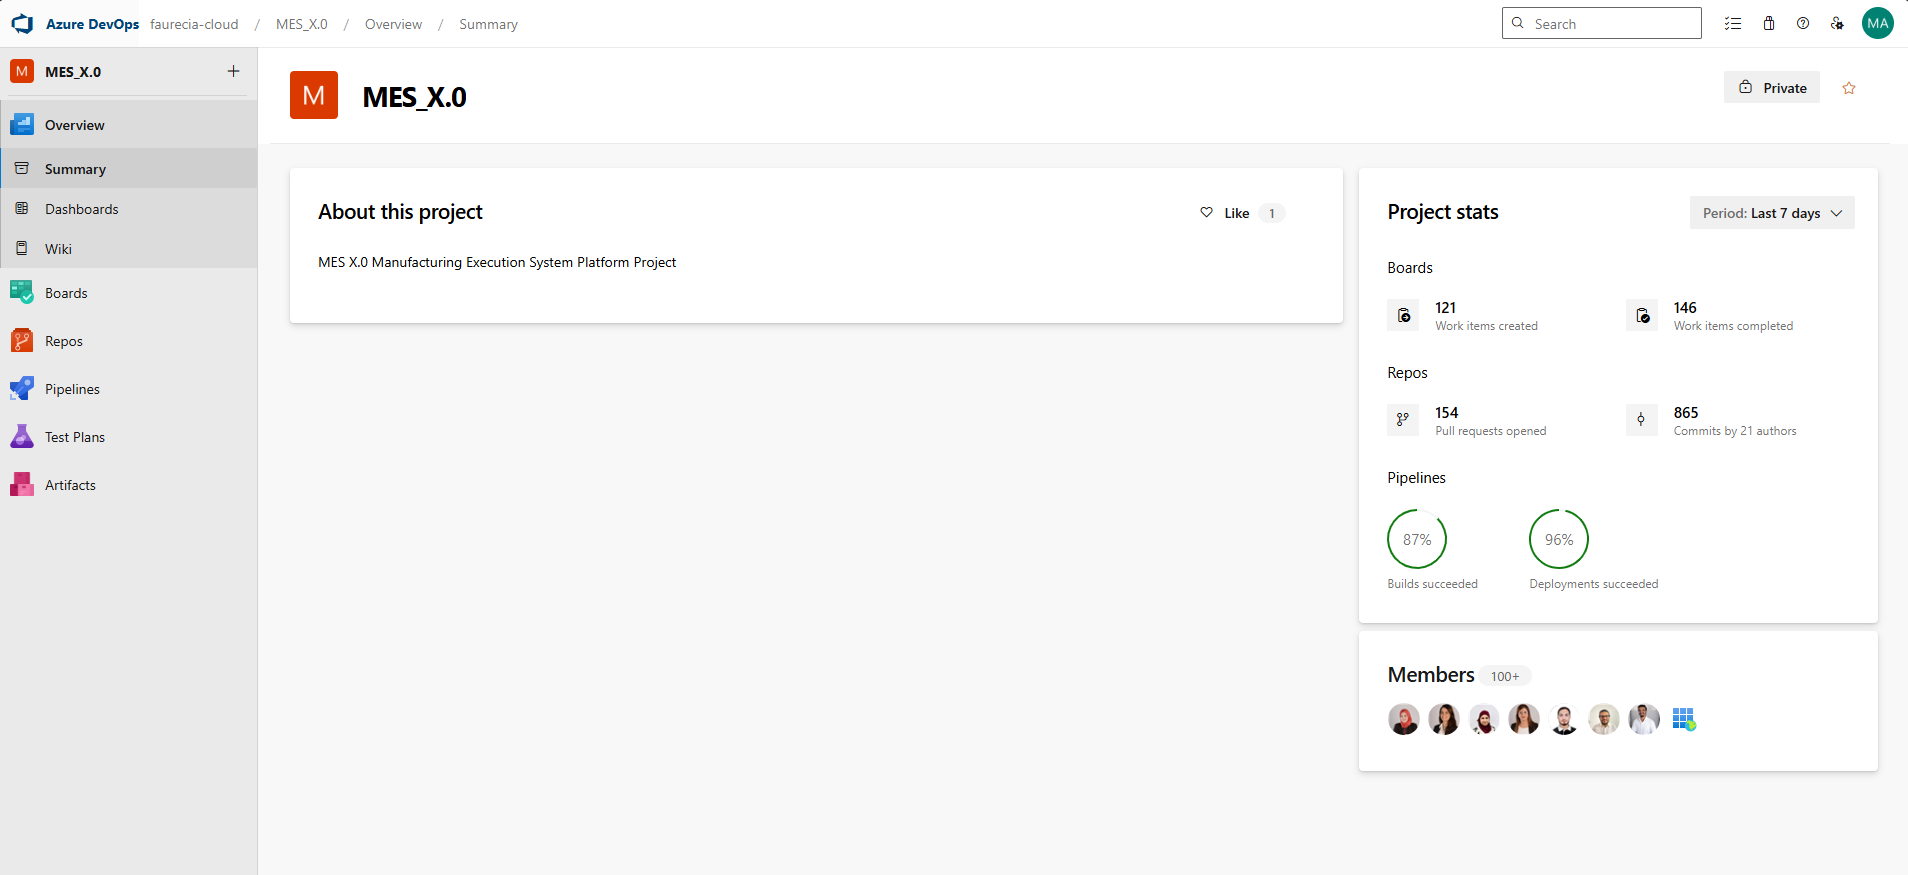
\includegraphics[width=0.95\linewidth]{img/overview/azure_board.png}
\caption{Azure DevOps environment used within the MES X.0 division, showing work item tracking and development workflow management}
\label{fig:azure-devops-board}
\end{figure}
\subsection{The Traceability Challenge}
\label{subsec:traceability-challenge}

In this multi-service, high-velocity development environment, a single
user-facing requirement — expressed as a work item at the Epic or Feature level
in Azure DevOps — typically decomposes into dozens of lower-level tasks, each
of which produces its own chain of development artifacts: a branch, one or more
commits, a pull request, and eventually a repository tag when the change is
released.

Understanding the complete impact of a requirement — or conversely, understanding
what requirements are affected by a change in a specific repository — requires
navigating this artifact chain in its entirety. For a release engineer
preparing a production deployment, this means answering questions such as:

\begin{itemize}
  \item Which work items are included in this release, and are they all in a
  completed state?
  \item For each work item, which pull requests carried the implementation, and
  in which repositories?
  \item For each repository, which commits were produced, and do they appear
  before or after the relevant release tag?
  \item Are there any commits that straddle a release boundary — present in one
  environment but not yet in another?
\end{itemize}

Before this project, answering these questions required a \textbf{manual and
entirely ad-hoc process}. The release engineer or developer would begin from a
work item in Azure DevOps, navigate to its linked pull requests, open each PR
to identify the target repository, navigate to the repository's commit history,
search for the relevant commits, check branch and tag references, and then
repeat the entire sequence for every related work item. Data extracted at each
step was typically recorded manually in spreadsheets to maintain a working
reference.

This process presented several critical limitations:

\begin{itemize}
  \item \textbf{Time cost}: a complete dependency trace for a single feature
  involving multiple services could require an entire working day to complete
  manually.
  \item \textbf{Error proneness}: the manual correlation of data across multiple
  Azure DevOps interfaces introduced a significant risk of missed links,
  incorrect associations, and incomplete coverage.
  \item \textbf{Non-reproducibility}: two engineers performing the same trace
  independently could arrive at different results depending on the path they
  followed and the data they chose to record.
  \item \textbf{Scalability failure}: as the number of microservices grew and
  development velocity increased, the manual approach became increasingly
  impractical, consuming disproportionate engineering time during critical
  release preparation phases.
\end{itemize}

\subsection{Project Motivation}
\label{subsec:motivation}

These limitations created a clear and urgent need for an automated solution.
The \textbf{MES-X Dependency Management} project was initiated within the
MES X.0 division to address this need directly: to design and implement a
system that would automate the reconstruction of dependency chains across Azure
DevOps artifacts, transforming a time-consuming and error-prone manual process
into a fast, reliable, and reproducible analytical capability.

The project was scoped as an end-of-study internship project, representing an
opportunity to deliver genuine industrial value while applying and extending
the software engineering knowledge acquired during the academic program.

% ─────────────────────────────────────────────────────────────────────────────
\section{Project Description}
\label{sec:project-description}

\subsection{Project Objectives}
\label{subsec:objectives}

The primary goal of the MES-X Dependency Management project is to design and
implement an \textbf{automated dependency traceability system} that replaces
the existing manual process with a reliable, efficient, and scalable solution
integrated into the Azure DevOps ecosystem.

The project pursues the following specific objectives:

\subsubsection{Automated Microservice Tag Identification}

The system must automatically identify and associate the relevant microservice
repository tags with work items by analyzing commit history and repository
metadata. This capability eliminates the need for manual navigation through
repository tag lists and commit histories, and ensures that the release context
of each code change is determined programmatically and consistently.

\subsubsection{Comprehensive Dependency Mapping}

The system must construct and expose complete traceability links across the full
chain of development artifacts: from high-level work items through pull requests
and commits down to repository branches and tags. This mapping must be complete
— covering all levels of the work item hierarchy and all artifact types — and
consistent across successive analysis sessions.

\subsubsection{Significant Reduction of Manual Effort}

By automating data retrieval, traversal, normalization, and aggregation, the
system must reduce the time required to perform a complete dependency analysis
from hours to seconds. This reduction must be sustained even for complex
analysis scenarios involving multiple work items and many repositories.

\subsubsection{Improved Data Accuracy and Consistency}

The system must eliminate the class of errors introduced by manual data
extraction and correlation. All dependency data must be derived from the same
authoritative source — the Azure DevOps APIs — through a standardized and
reproducible process, ensuring that results are accurate and identical across
successive runs for the same input.

\subsubsection{End-to-End Traceability}

The system must enable a user to trace any work item from its initial
description to the exact commits and microservice tags it affected, entirely
within a single analysis session. No cross-tool navigation or manual correlation
should be required to obtain a complete dependency view.

\subsubsection{Reusable and Scalable Architecture}

The system must be built on a modular, maintainable architecture that can be
extended to support additional artifact types, additional analysis modes, or
integration into other Forvia digital platforms — without requiring a
fundamental redesign of the existing system.

\subsection{Technical Scope}
\label{subsec:technical-scope}

The project encompasses the design and implementation of three interconnected
technical components: a backend service, a frontend application, and an
Azure DevOps integration layer.

\subsubsection{Backend Development}

The backend was developed using \textbf{NestJS} with TypeScript, a framework
chosen for its native support of modular architecture, dependency injection,
and TypeScript-first development — properties well-suited to the clean,
maintainable design required by this project.

The backend's responsibilities include:

\begin{itemize}
  \item Secure integration with the Azure DevOps REST APIs using Personal Access
  Token authentication.
  \item Normalization of raw Azure DevOps responses into structured, typed Data
  Transfer Objects that form the stable internal data model of the system.
  \item Recursive traversal of work item dependency graphs across multiple
  hierarchy levels and relation types.
  \item Resolution of pull requests, commits, repository branches, and Git tags
  for each node in the dependency graph.
  \item Implementation of batch processing strategies to minimize API call
  volume and respect rate limits.
  \item Implementation of Server-Sent Events streaming for progressive delivery
  of large analysis results.
  \item Exposure of well-documented RESTful endpoints, complemented by
  interactive Swagger documentation for developer exploration and testing.
\end{itemize}

\subsubsection{Frontend Application}

The frontend was developed using \textbf{Vue 3} with the Quasar framework,
providing a production-grade, responsive interface for initiating and exploring
dependency analyses. The frontend's role is not limited to presentation: it
actively participates in the orchestration of analysis sessions by managing
asynchronous backend calls, assembling view state from streamed results, and
providing real-time progress feedback to the user.

Key features of the frontend include:

\begin{itemize}
  \item Interactive visualization of work item dependency graphs, presenting
  hierarchical relationships, pull request links, and commit references in a
  structured and navigable form.
  \item Real-time batch processing interface powered by Server-Sent Events,
  allowing users to observe analysis progress incrementally rather than waiting
  for a single blocking response.
  \item Clear presentation of relationships between work items, pull requests,
  commits, branches, and tags, organized by repository and analysis mode.
  \item A dedicated Decision Dashboard that presents the release classification
  output of the aggregation component in an actionable, decision-ready format.
  \item A responsive and operationally focused design, tailored for everyday
  use by release engineers and development team leads.
\end{itemize}

\subsubsection{Azure DevOps Integration and Data Processing}

The solution relies on the Azure DevOps REST API as its exclusive data source.
The integration layer is responsible for all communication with this external
system and implements several mechanisms to ensure reliability and efficiency:

\begin{itemize}
  \item Authentication via Personal Access Tokens with secure credential
  management.
  \item Intelligent batching and concurrency control to respect Azure DevOps
  API rate limits during high-volume analysis sessions.
  \item A robust dependency resolution engine capable of recursive graph
  traversal, entity deduplication, and cross-module result normalization.
  \item Structured error handling and retry logic for transient API failures,
  ensuring that partial external failures do not silently corrupt analysis
  results.
\end{itemize}

\subsection{Project Activities}
\label{subsec:activities}

The project followed a structured development lifecycle organized around the
following phases:

\begin{itemize}
  \item \textbf{Requirements Analysis}: study of the existing manual
  traceability workflow, interviews with release engineers and developers, and
  formalization of the system's functional and non-functional requirements.

  \item \textbf{System Design and Architecture}: definition of the three-layer
  architecture, identification of the four main backend components, design of
  API contracts and data transfer objects, and preparation of the frontend
  structure.

  \item \textbf{Backend Implementation}: development of the Azure DevOps
  integration layer, recursive traversal logic, pull request resolution,
  commit and tag processing services, and progressive streaming support.

  \item \textbf{Frontend Development}: implementation of the main analysis
  views, centralized state management with Pinia, integration of real-time SSE
  updates, and development of the Decision Dashboard.

  \item \textbf{Testing and Validation}: unit testing of backend services and
  utilities, validation of backend contracts against frontend needs, and
  end-to-end checks for the main analysis scenarios.

  \item \textbf{Integration and Optimization}: performance tuning of graph
  traversal and batch resolution, implementation of in-memory caching, and
  verification of result consistency across analysis modes.

  \item \textbf{Deployment Preparation}: backend containerization with Docker,
  environment configuration, CI/CD pipeline setup, and completion of Swagger
  documentation for developer handoff.
\end{itemize}

% ─────────────────────────────────────────────────────────────────────────────
\section{Conclusion}
\label{sec:overview-conclusion}

This chapter has presented the industrial setting of the MES-X Dependency
Management project and clarified why dependency tracing had become a real
operational issue. In a large microservices ecosystem, manual analysis no
longer provides the speed, consistency, or reliability required for release
preparation.

The next chapter translates that problem into a formal requirements
specification. It defines what the system must deliver functionally and which
quality constraints it must satisfy in practice.
\newpage

%% ── Chapter 2 — Study of Existing Solutions ─────────────────────────────────
\chapter{Study of the Existing}
\label{chap:existing}

\section{How Dependency Tracking Is Done Today}

This chapter examines the manual process used before the introduction of the
MES-X Dependency Management system. Understanding that workflow is important,
because the design choices made later in the report are direct responses to its
limitations.

In the MES X.0 environment, the starting point is usually a \textbf{user
story} in Azure DevOps. That story is often linked to several child tasks, and
each task may produce its own pull request, commits, and release references in
different repositories. Azure DevOps stores all of these artifacts, but it does
not provide a single consolidated view of their dependency chain.

In practice, a developer preparing a dependency report had to repeat the same
sequence for \emph{each} user story under analysis:

\begin{enumerate}
    \item Open the work item in Azure DevOps and note all linked child tasks and related
          items.
    \item Navigate to the \textbf{Development} panel of each item to find associated
          pull requests.
    \item Open every pull request individually, then switch to its \textbf{Commits} tab.
    \item Inspect each commit message and the list of changed files to identify which
          microservice is affected and extract any version tags present in the commit.
    \item Record the collected information---work item ID, PR number, commit hash,
          microservice name, tag---row by row in an Excel spreadsheet.
    \item Repeat the entire sequence for every child work item linked to the original
          story.
\end{enumerate}

During a typical sprint, with ten to fifteen user stories and several pull
requests per story, this work could easily occupy most of a day. Every link had
to be opened manually, and every relevant tag had to be checked one by one.

\section{Illustrative Example}

Consider a user story such as \emph{``Update shared configuration service for
plant B.''} The change may involve the configuration service itself, a dependent
API gateway, and a deployment adjustment. In practice, that single story can be
split into several child tasks, each with its own pull request and its own set
of commits.

To build a dependency view for that story, the developer must inspect each pull
request, identify the affected repository, review the associated commits, and
locate the relevant release tags. Even in a modest case, this means opening
several pull requests and reading through dozens of commits. Once this effort is
multiplied across a full sprint, the workload becomes substantial and the risk
of omission increases.

\section{Limitations and Their Consequences}

The manual process creates four major problems.

\textbf{Time consumption.} Preparing a complete dependency report for a sprint
can take from several hours to a full working day. That time is repeatedly
spent on navigation and transcription instead of implementation or review.

\textbf{High error risk.} The result depends on careful human inspection. A
single missed commit, an overlooked repository, or an incorrect tag reference
can produce an incomplete report and lead to poor release decisions.

\textbf{Poor scalability.} The MES X.0 platform already contains many
microservices, and its scope continues to grow. As more repositories are added,
the manual approach becomes less realistic and more costly.

\textbf{Lack of a shared source of truth.} Because the final result is often
stored in spreadsheets, two engineers can produce different analyses for the
same feature with no automatic way to reconcile the difference.

These limitations affect both productivity and reliability. They justify the
need for a structured, automated solution, which is formalized in the next
chapter through the system requirements.
\newpage

%% ── Chapter 3 — Requirements Analysis ──────────────────────────────────────
% ============================================================================
% CHAPTER 3  REQUIREMENTS SPECIFICATION
% ============================================================================

\chapter{Requirements Specification}
\label{chap:requirements}

% 
\section{Introduction}
\label{sec:req-intro}

This chapter describes what the MES-X Dependency Management system must do and
how well it must do it. The goal at this stage is to describe the expected
behavior independently of implementation choices, so the architecture and code
can later be measured against a clear baseline.

The requirements come from studying the manual workflow described in the
previous chapter, talking with developers and release engineers, and watching
traceability tasks being carried out in the MES X.0 environment. They cover
both what the system must do and the quality bar it must meet in daily use.


% 
\section{Functional Requirements}
\label{sec:functional-requirements}

The functional requirements define the main capabilities of the MES-X Dependency Management system.
They describe how the system processes Azure DevOps data to build a complete traceability view across work items, source code, and release information.

\begin{itemize}

\item \textbf{FR-01  Pull Request Resolution} \\
The system shall retrieve pull requests from Azure DevOps and associate them with their corresponding work items.  
This enables the system to establish a consistent link between work tracking elements and source control changes, which forms the entry point of the traceability pipeline.
\item \textbf{FR-02  Commit and Tag Contextualization} \\
The system shall extract commits linked to each pull request and add contextual information, including branch details and repository tags.  
This contextual information is required to determine the position of each change within the release lifecycle and to support release-level analysis.

\item \textbf{FR-03  Dependency Graph Construction} \\
The system shall construct a dependency graph starting from one or multiple root work items.  
It shall traverse all related entities through Azure DevOps relationships, including parent-child links, pull request associations, and commit references, in order to reconstruct the full dependency chain.

\item \textbf{FR-04  Aggregation and Decision Output} \\
The system shall aggregate all retrieved entities into a unified data model.  
This includes normalization of work items, pull requests, and commits, as well as removal of duplicates caused by multi-path traversal.  
The final output shall provide a structured view that supports release analysis and decision-making.

\item \textbf{FR-05  End-to-End Read-Only Traceability} \\
The system shall provide a complete traceability view across all relevant artifact levels: work items, pull requests, commits, branches, and tags.  
All interactions with Azure DevOps shall be strictly read-only, ensuring that no modification, creation, or deletion of external data is performed by the system.
\item \textbf{FR-06  Sprint-Based and Multi-Sprint Dependency Resolution} \\
The system shall support dependency analysis starting from one or more sprints, as well as from work items belonging to multiple sprints.  
It shall retrieve all related work items and trace their dependencies across pull requests, commits, and repository versions.

The system shall also identify the corresponding release versions associated with these work items in order to support validation of transitions between environments (e.g., development, pre-production, production).  
This enables the system to determine which changes are required to move a set of work items to the next environment.
\end{itemize}
\section{Non-Functional Requirements}
\label{sec:nonfunctional-requirements}

Non-functional requirements define the quality attributes that the system must respect to operate correctly in an industrial MES X.0 environment. They ensure that the system is not only functionally correct, but also performant, scalable, reliable, maintainable, and secure.

In this project, each non-functional requirement was directly translated into implementation decisions within the system architecture. Their validation was performed using a combination of unit tests, integration tests, runtime observation, and deployment-level verification.

% 
\subsection{Performance}

Performance ensures efficient dependency analysis even in large-scale distributed data.

\begin{itemize}

\item \textbf{NFR-PE-01  Graph Traversal Efficiency}:  
The system uses graph traversal strategies in the backend to explore relationships between work items, pull requests, and commits while avoiding redundant exploration. This requirement is supported by the Work Item and Commit services, which combine traversal logic with in-memory deduplication and visited-state management.

This requirement was verified through service-level tests and runtime observation of traversal behavior during dependency analysis.

\item \textbf{NFR-PE-02  API Call Optimization}:  
Azure DevOps API requests are optimized through batching and controlled concurrency. In particular, the backend uses the \texttt{p-limit} library to cap concurrent external calls in traceability-critical services such as work item traversal, commit resolution, and tag resolution.

This behavior was verified through code-level inspection of the concurrency control implementation, unit tests around the affected services, and runtime observation showing reduced request bursts and more stable execution.

\item \textbf{NFR-PE-03  Caching and Deduplication}:  
Processed entities are cached and deduplicated during traversal to avoid recomputation and repeated API calls. This is implemented through local caches, aggregation normalization, and repository-level deduplication utilities in the backend.

Its effectiveness was verified through repeated executions on identical inputs, which produced stable outputs with lower redundant processing.

\item \textbf{NFR-PE-04  Progressive Feedback}:  
Long-running operations provide streaming updates to the frontend, improving perceived responsiveness. This is implemented through Server-Sent Events, with a dedicated streaming service that emits progressive batches using the \texttt{text/event-stream} protocol.

This requirement was validated through end-to-end execution of batch analysis scenarios in which the frontend received progressive updates before full completion.

\end{itemize}

% 
\subsection{Scalability}

Scalability ensures the system can handle increasing data volume and repository complexity.

\begin{itemize}

\item \textbf{NFR-SC-01  Algorithmic Scalability}:  
The combination of graph traversal, caching, and controlled concurrency ensures that execution cost grows with the actual dependency graph size rather than with redundant repeated exploration.

This was verified through multi-root and sprint-based analysis scenarios involving multiple work items and repositories.

\item \textbf{NFR-SC-02  Microservices Architecture}:  
The system is divided into domain-focused backend services and modules, including Work Item, Pull Request, Commit, Sprint, Decision, and LLM modules. This modular NestJS architecture supports isolated evolution, clearer responsibilities, and future scaling of the processing pipeline.

This was verified during implementation by integrating new modules without redesigning the existing traceability flow.

\item \textbf{NFR-SC-03  Containerized Deployment}:  
Docker is used to package both backend and frontend applications, ensuring reproducible builds and deployment behavior across environments.

This was verified through the presence of Docker build scripts and Dockerfiles in both applications, as well as their integration into the delivery workflow.

\item \textbf{NFR-SC-04  Dapr Integration}:  
Dapr is used as an integration component for secret retrieval and distributed application support. In the current solution, it is concretely used to retrieve Azure DevOps secrets from the configured secret store and it prepares the platform for wider distributed-service evolution.

This was verified through the implemented backend integration based on \texttt{DaprClient} and the application configuration services.

\end{itemize}

% 
\subsection{Reliability}

Reliability ensures consistent system behavior under all execution conditions.

\begin{itemize}

\item \textbf{NFR-RE-01  Deterministic Output}:  
The system is designed to produce identical results for identical inputs regardless of execution order. This is supported by deterministic normalization, deduplication rules, and stable aggregation logic in the backend.

This requirement was verified through repeated runs using the same inputs and by checking that the resulting traceability outputs remained consistent.

\item \textbf{NFR-RE-02  Fault Isolation}:  
Failures in Azure DevOps API calls are isolated within the backend integration and service layers to avoid uncontrolled propagation across the whole application.

This is supported by dedicated service boundaries, exception handling, and structured logging in the NestJS backend.

\item \textbf{NFR-RE-03  Retry Mechanism}:  
Transient failures are handled using controlled recovery logic and guarded external-call handling while preserving partial processing whenever possible.

This was verified through service tests and runtime observation of backend behavior during unstable or partial-response situations.

\item \textbf{NFR-RE-04  Data Consistency}:  
All processed entities remain consistent across transformation and aggregation stages. This is supported by DTO-based contracts, typed mapping, and centralized aggregation logic.

This requirement was verified through unit tests, API checks, and frontend-backend consistency validation during traceability workflows.

\end{itemize}

% 
\subsection{Maintainability}

Maintainability ensures the system remains easy to evolve and extend.

\begin{itemize}

\item \textbf{NFR-MA-01  Modular Design}:  
Each module follows a modular design aligned with the Single Responsibility Principle, ensuring clear separation of concerns between traversal, commit processing, sprint handling, decision aggregation, and LLM review.

This was verified during development by the existence of dedicated backend modules and services with isolated responsibilities.

\item \textbf{NFR-MA-02  Clean Architecture}:  
Business logic, API integration, and data processing layers are separated to improve readability, testability, and long-term evolution. This separation is reflected in the NestJS service structure and in the dedicated configuration, integration, and utility layers.

This requirement was verified through code review, module boundaries, and the ability to test controllers and services independently.

\item \textbf{NFR-MA-03  Reusable Components}:  
Core services are designed to be reusable across multiple MES modules. Examples include shared streaming, logging, Azure DevOps integration, and aggregation utilities.

This was verified by reuse of common services across several backend domains.

\item \textbf{NFR-MA-04  Standardization}:  
Consistent naming conventions, DTO contracts, linting rules, and formatting rules are enforced across the codebase. This is supported by ESLint, Prettier, and typed DTO usage in both backend and frontend projects.

This requirement was verified through lint scripts, formatting scripts, and the standardized project structure used during implementation.

\end{itemize}

% 
\subsection{Security and Data Integrity}

Security ensures controlled and safe access to industrial data.

\begin{itemize}

\item \textbf{NFR-SE-01  Token-Based Authentication}:  
Azure DevOps access is secured using Personal Access Tokens whose secret names are provided through configuration and resolved at runtime from the secret store. The PAT is handled only by the backend and is never exposed to the frontend.

This requirement was verified through the implemented Azure DevOps connection service, which retrieves the secret through Dapr before creating the authenticated Azure DevOps client.

\item \textbf{NFR-SE-02  Frontend Route Protection}:  
The frontend includes a route-protection mechanism based on Vue Router metadata, a global \texttt{beforeEach} navigation guard, and an unauthorized fallback page. This mechanism allows views to be protected whenever \texttt{requiresAuth} is enabled.

This was verified through the implemented authentication and authorization flow in the frontend router and authentication store.

\item \textbf{NFR-SE-03  Secret Management}:  
Sensitive credentials are managed through secure configuration mechanisms using \texttt{ConfigService}, environment variables, and Dapr secret store integration.

This was verified through the backend configuration modules and runtime secret resolution logic.

\item \textbf{NFR-SE-04  Backend-Only External Access}:  
All communication with Azure DevOps is handled exclusively by the backend layer through dedicated integration services. The frontend communicates only with backend endpoints and does not directly call Azure DevOps.

This requirement was verified through the architecture, the implemented router/API flow, and the backend integration services.

\item \textbf{NFR-SE-05  Read-Only Policy}:  
The system is strictly read-only with respect to Azure DevOps, ensuring that no external artifacts are created, modified, or deleted during traceability analysis.

This was verified by reviewing the exposed backend functionality, which focuses on retrieval, traversal, enrichment, and aggregation only.

\end{itemize}
\subsection{Verification Scope}

This chapter defines the non-functional targets and the technical mechanisms
used to satisfy them. The concrete execution evidence (test outcomes,
deployment traces, and pipeline-level proof) is consolidated in the
Implementation chapter to avoid redundancy and keep this specification focused
on requirements and verification criteria.

\section{Use Case Model}
\label{sec:use-case-model}

The use case model shows how the actors interact with the system to carry out
traceability and analysis tasks. It complements the requirement lists with a
behavioral view of the system.

\subsection{Actors}
\label{subsec:actors}

The use case diagram highlights the two primary actors shown in the figure:
a Developer and an LLM Provider. The diagram is intended to make the main
workflow and intelligence flow visible at a glance.

\subsubsection{Developer and Release Engineer}

The primary user. Developers use the system to understand the impact of a work
item on the codebase. Release engineers use it to check release scope and
confirm whether changes sit on the correct side of a release boundary.

This actor starts analysis sessions, chooses the analysis mode, reviews
results, and uses the Decision Dashboard output to support release,
integration, and escalation decisions.

\subsubsection{LLM Provider}

An external AI service used by the system to review commits and generate
intelligent insights. This actor supports the "Review Commit with LLM" use
case and is shown in the diagram as a cross-cutting service.

\subsubsection{Additional Actors}

Other actors are part of the overall model but are not illustrated in this
view. The Administrator manages operational configuration and availability,
and Azure DevOps is the external data source for work items, pull requests,
commits, branches, and tags.

\subsection{Use Case Descriptions}
\label{subsec:use-cases}

The following use cases describe what the system does from each actor's
perspective.

\subsubsection{Work Item Use Cases}

\begin{itemize}
  \item \textbf{UC-01  Analyze Single Work Item}: The user provides one work item ID. The system traverses the full dependency graph, resolves related pull requests and commits, enriches commits with branch and tag context, and returns a complete normalized trace result.

  \item \textbf{UC-02  Analyze Multiple Work Items}: The user provides several work item IDs. The system traverses each root, merges and deduplicates the results, and returns one consolidated trace. This supports release scope analysis across a sprint or milestone.

  \item \textbf{UC-03  Stream Work Item Tasks}: The user starts a batch analysis session. The system streams resolved work item tasks progressively so progress is visible in real time, and items can be selected for further analysis before the full dataset has loaded.
\end{itemize}

\subsubsection{Pull Request Use Cases}

\begin{itemize}
  \item \textbf{UC-04  Retrieve Pull Request Work Items}: Given a pull request identifier, the system returns the work items formally linked to that PR on the Git side, along with the normalized PR summary including the repository name.
\end{itemize}

\subsubsection{Commit Use Cases}

\begin{itemize}
  \item \textbf{UC-05  Retrieve Commits by Work Item}: Given a work item ID, the system returns the deduplicated list of commits linked to that item, resolved through direct links and pull request expansion.

  \item \textbf{UC-06  Retrieve Commits by Pull Request}: Given a pull request ID, the system returns the list of commits merged as part of that PR.

  \item \textbf{UC-07  List Repository Branches and Tags}: Given a repository ID, the system returns the available branch and tag references needed to interpret commit positions.

  \item \textbf{UC-08  Resolve Commit Tag Context}: Given a repository and a commit, the system determines the most recent tag reachable from that commit on the relevant branch.

  \item \textbf{UC-09  Batch Resolve Commit Tag Context}: Given a repository and multiple commits, the system resolves the tag context of all specified commits in one operation to reduce API usage on large graphs.
\end{itemize}

\subsubsection{Aggregation and Decision Use Cases}

\begin{itemize}
  \item \textbf{UC-10  Generate Dependency View}: After a trace is complete, the system aggregates all collected data — work items, pull requests, commits, and tag context — into a single decision-ready view. Work items are grouped by completion state and repositories are classified by their commit position relative to the target release.

  \item \textbf{UC-11  Configure System}: The Administrator updates environment-level configuration, including Azure DevOps connection settings, API credential management, and deployment parameters.
\end{itemize}

\subsection{Use Case Diagram}
\label{subsec:use-case-diagram}

Figure~\ref{fig:usecase-diagram} shows the complete use case diagram, with the
primary actors and all eleven use cases.

\vspace{0.5em}
\hspace{0em}

\begin{figure}[H]
  \centering
  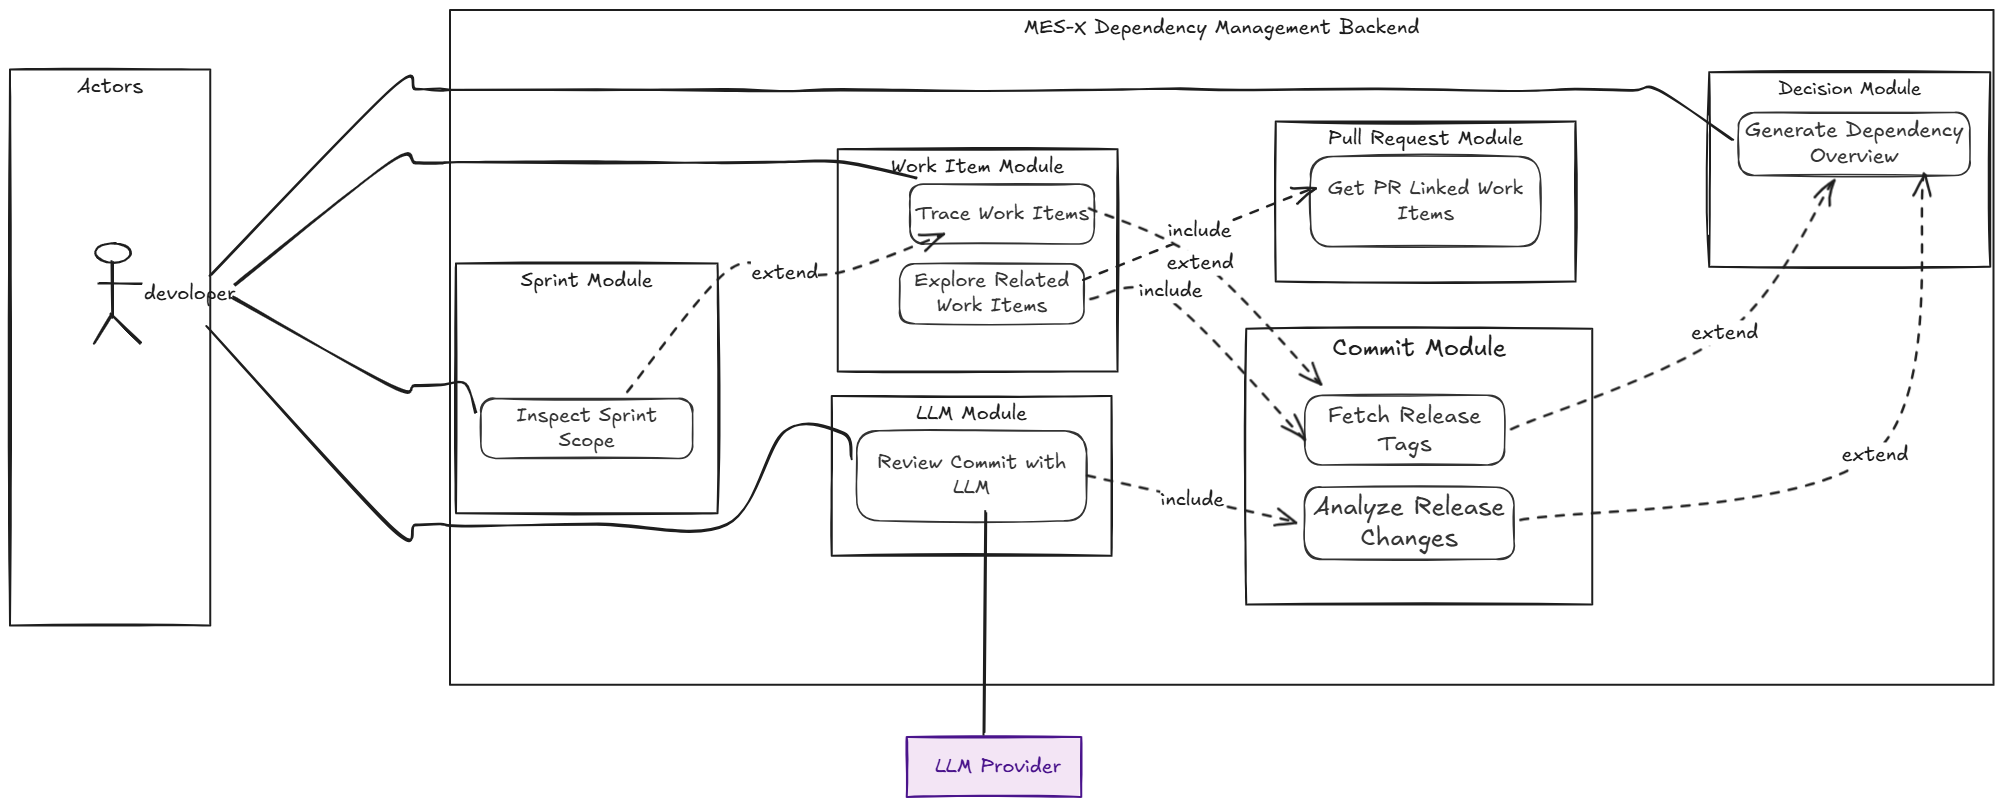
\includegraphics[width=1\textwidth,height=0.8\textheight,keepaspectratio]{img/archi/use_case.png}
  \caption{Use Case Diagram of the MES-X Dependency Management System.}
  \label{fig:usecase-diagram}
\end{figure}

\subsection{Scope Boundaries}
\label{subsec:scope-boundaries}

Two boundaries are worth stating clearly.

First, as set out in \textbf{FR-05}, all use cases are read-only. The system
does not create, modify, or delete anything in Azure DevOps. Azure DevOps
appears in the model only as a data source.

Second, notification and alerting features, mentioned in some internal notes as
possible future additions, are out of scope here. This specification covers
only the traceability and analysis capabilities described above.

% 
\section{Requirements Traceability Summary}
\label{sec:req-traceability}

Table~\ref{tab:req-traceability} shows how each functional requirement group
maps to a system component. This makes clear which part of the system is
responsible for which requirements, and creates the link between specification
and design.

\begin{table}[H]
  \centering
  \caption{Functional Requirements to System Component Traceability Matrix}
  \label{tab:req-traceability}
  \begin{tabular}{|p{4.5cm}|p{3cm}|p{5.5cm}|}
    \hline
    \textbf{Requirement Group} & \textbf{Requirement IDs} & \textbf{Responsible Component} \\
    \hline
    Pull Request Resolution & FR-01 & Pull Request Resolution Component \\
    \hline
    Commit and Tag Contextualization & FR-02 & Commit Aggregation Component \\
    \hline
    Dependency Graph Construction & FR-03 & Work Item Management Component \\
    \hline
    Aggregation and Decision Output & FR-04 & Decision Aggregation Component \\
    \hline
    End-to-End Read-Only Traceability & FR-05 & All components, Trace UI \\
    \hline
    Sprint-Based and Multi-Sprint Resolution & FR-06 & Sprint + Work Item + Commit Components \\
    \hline
  \end{tabular}
\end{table}

% 
\section{Conclusion}
\label{sec:req-conclusion}

This chapter set out the full requirements for the MES-X Dependency Management
system. The functional requirements cover five areas: work item traceability,
pull request resolution, commit enrichment, data aggregation, and analytical
reporting. The non-functional requirements set the bar for performance,
scalability, reliability, maintainability, and security. The use case model
translates those requirements into eleven concrete actor-system interactions.

Together, these requirements form the reference baseline for the rest of the
report. They define not just what the system must do, but the level of
performance, reliability, and maintainability expected of it in real use.

The next chapter presents the proposed architecture and explains how the chosen
design addresses these requirements through a layered structure and a
specialized traceability pipeline.
\newpage

%% ── Chapter 4 — Proposed Solution ──────────────────────────────────────────
% ═══════════════════════════════════════════════════════════════════════════════
% CHAPTER — PROPOSED SOLUTION
% End-of-Study Report — MES-X Dependency Traceability System
% ═══════════════════════════════════════════════════════════════════════════════

\chapter{Proposed Solution}
\label{chap:proposed-solution}

% ─────────────────────────────────────────────────────────────────────────────
\section{Introduction}
\label{sec:solution-intro}

The previous chapter showed that Azure DevOps stores the necessary traceability
data, but does not present it in a form that is easy to analyze end to end.
Teams therefore have to move manually between work items, pull requests,
commits, branches, and tags to reconstruct the dependency chain of a feature.
That approach is workable on a small scale, but it becomes costly and unreliable
in a large microservices environment.

The proposed solution addresses this gap through a \textbf{centralized
dependency traceability system} designed for Azure DevOps-based workflows.
Rather than replacing the existing platform, it adds an analytical layer on top
of it: the system retrieves data from Azure DevOps APIs, rebuilds dependency
graphs, enriches the raw artifacts with additional context, and exposes the
result through a dedicated interface.

The system is built around three guiding ambitions:

\begin{itemize}
  \item \textbf{Completeness}: Every artifact in the dependency chain — from
  epics and features down to individual commits and Git tags — must be
  reachable and traceable within a single analysis session.

  \item \textbf{Consistency}: All data must be normalized before processing so
  that results are stable and predictable regardless of the structural
  variations present in Azure DevOps API responses.

  \item \textbf{Actionability}: The final output must not be a raw data dump.
  It must be organized into structured, decision-ready views that directly
  support release readiness assessment, impact analysis, and dependency
  validation.
\end{itemize}

The following sections present the global architecture of the solution, the
design principles that govern its construction, the four core components that
form the traceability pipeline, the end-to-end data flow connecting them, and
the concrete advantages the system delivers over the current state of practice.


% ─────────────────────────────────────────────────────────────────────────────
\section{Global System Architecture}
\label{sec:global-architecture}

The system adopts a \textbf{three-layer architecture} that cleanly separates
the concerns of user interaction, business orchestration, and external data
access. This separation is not merely a structural convention: it is a
deliberate design decision that ensures each layer can be developed, tested,
and evolved independently without creating cascading changes across the system.

\begin{figure}[htbp]
  \centering
  
\includegraphics[width=\linewidth]{img/archi/general_archi.png}
  \caption{Global three-layer architecture of the proposed solution.}
  \label{fig:global-architecture}
\end{figure}

\subsection{Presentation Layer — Trace UI}
\label{subsec:presentation-layer}

The Presentation Layer is the entry point for end users. It is implemented as a
dedicated web interface — referred to throughout this document as the
\emph{Trace UI} — that allows users to initiate dependency analysis sessions,
monitor their progress in real time, and explore the resulting dependency graphs
and decision outputs.

The Trace UI is not a passive display surface. It actively participates in the
orchestration of the analysis by:

\begin{itemize}
  \item accepting user-defined analysis parameters (work item identifiers,
  project context, analysis mode);
  \item managing the lifecycle of asynchronous and streamed backend interactions;
  \item assembling and normalizing backend responses into a coherent view state;
  \item presenting structured, layered results across multiple specialized views.
\end{itemize}

The interface supports three distinct analysis modes — single work item trace,
batch work item trace, and batch-related work item trace — each tailored to
a specific use case and level of analytical depth.

\subsection{Application Layer — Backend Services}
\label{subsec:application-layer}

The Application Layer constitutes the analytical core of the system. It is
implemented as a modular backend service responsible for orchestrating all
traceability logic: dependency graph traversal, data normalization, cross-module
enrichment, and decision aggregation.

This layer receives structured requests from the Trace UI, coordinates calls to
the Azure DevOps APIs, applies domain-specific processing rules, and returns
normalized, enriched results through well-defined API contracts. It acts as the
intermediary that isolates the Presentation Layer from the complexity and
variability of the underlying data source.

The Application Layer is internally composed of four specialized components —
each described in detail in Section~\ref{sec:core-components} — that together
form a sequential traceability pipeline.

\subsection{Integration Layer — Azure DevOps REST APIs}
\label{subsec:integration-layer}

The Integration Layer represents the external data source of the system. Azure
DevOps REST APIs serve as the single source of truth for all project artifacts:
work items and their hierarchical relations, pull request metadata and linked
work items, commit histories, repository branch structures, and Git tag
references.

The system interacts with two distinct Azure DevOps API surfaces:

\begin{itemize}
  \item \textbf{Work Item Tracking API}: used to retrieve work items, resolve
  parent/child and linked-item relationships, and query work item states and
  metadata.
  \item \textbf{Git API}: used to retrieve pull request details, commit
  histories, branch references, and tag context for specific commits and
  repositories.
\end{itemize}

All interactions with these APIs are encapsulated within a dedicated integration
utility layer that handles authentication, request formatting, response
normalization, and error management. This encapsulation ensures that the rest
of the system never directly depends on the raw Azure DevOps response structures,
protecting the application against API changes and simplifying future migrations.

\subsection{Interaction Between Layers}
\label{subsec:layer-interaction}

The three layers interact through a strict unidirectional flow. The Presentation
Layer communicates only with the Application Layer, while the Application Layer
handles all interactions with Azure DevOps through the Integration Layer. The
frontend never accesses Azure DevOps directly.

This separation keeps responsibilities clear. Changes in external APIs remain
isolated in the integration utilities, business rules stay concentrated in the
backend, and each layer can be tested independently with controlled inputs and
outputs.


% ─────────────────────────────────────────────────────────────────────────────
\section{Design Principles}
\label{sec:design-principles}

The architecture of the proposed solution is governed by four fundamental design
principles. These principles were not chosen arbitrarily: each one addresses a
specific category of risk or complexity identified during the problem analysis
phase, and each one shapes concrete decisions visible throughout the system
design.

\subsection{Modularity}
\label{subsec:modularity}

The system is decomposed into four focused, independent modules: Work Item
Management, Pull Request Resolution, Commit Aggregation, and Decision
Aggregation. Each module encapsulates a coherent set of responsibilities and
exposes its behavior exclusively through a well-defined API surface. No module
contains logic that properly belongs to another.

This modularity serves several practical purposes. First, it reduces the
cognitive complexity of each individual component, making the system easier to
understand and maintain. Second, it limits the impact of changes: a modification
to the commit resolution strategy, for example, requires changes only in the
Commit Aggregation module and does not cascade into the Work Item or Decision
modules. Third, it improves testability by allowing each module to be exercised
in isolation with controlled inputs.

\subsection{Separation of Concerns}
\label{subsec:separation-of-concerns}

Modules interact only through well-defined data contracts — specifically, through
typed Data Transfer Objects (DTOs) that specify the exact shape of data crossing
module boundaries. No module has direct knowledge of another module's internal
implementation, internal data structures, or external API dependencies.

This principle is particularly important in a system that depends on external
APIs with variable response structures. By ensuring that each module only
operates on normalized, contract-conformant data, the system avoids a class of
bugs that would otherwise arise from implicit assumptions about data shape. It
also ensures that each module's implementation can be refactored or replaced
without affecting its consumers, as long as the contract remains stable.

\subsection{Data Normalization}
\label{subsec:data-normalization}

All data received from Azure DevOps APIs is immediately transformed into
internal DTOs before being used in any processing logic. This normalization step
occurs at the boundary of the Integration Layer and is mandatory for every
response, regardless of the consuming module.

The purpose of this principle is to create a stable, homogeneous internal data
model that all system components can rely on. Azure DevOps API responses are
often heterogeneous: the same conceptual entity — such as a pull request link
embedded in a work item relation — may appear in different structural forms
depending on the API version, the repository configuration, or the type of
relation. Without normalization at the entry point, this heterogeneity would
propagate throughout the system and require every consuming component to handle
structural variability defensively.

Data normalization therefore acts as a \emph{complexity firewall}: it absorbs
the variability of the external world at the boundary and exposes a clean,
consistent model to the internal domain.

\subsection{Batch-Oriented Processing}
\label{subsec:batch-processing}

To support performance and scalability, the system favors batch API interactions
over individual, item-by-item calls whenever the data access pattern permits it.
Work item retrieval, commit resolution, and tag context lookup are all designed
around group operations: instead of issuing one API call per entity, the system
collects identifiers, groups them by natural boundaries (such as repository or
project), and issues a single grouped request.

This design principle is a direct response to two concrete challenges. First,
Azure DevOps APIs enforce rate limits that can be triggered by high volumes of
sequential individual requests during a large-scale analysis session. Second,
individual call patterns introduce significant latency through cumulative network
round-trip overhead, particularly when resolving tag context for dozens of
commits across multiple repositories.

By adopting a batch-oriented processing model throughout the pipeline, the system
reduces both the total number of API calls and the total elapsed time of an
analysis session, making it viable for large projects and portfolios.


% ─────────────────────────────────────────────────────────────────────────────
\section{Core Components}
\label{sec:core-components}

The Application Layer is internally organized into four specialized components
that together form a complete, sequential traceability pipeline. Each component
is responsible for a distinct stage of the analysis: from initial dependency
graph construction, through pull request and commit resolution, to final
decision aggregation. The components are designed to be composable — the output
of each stage becomes the input of the next — while remaining independently
testable and evolvable.

% ─────────────────────────────────────────────────────────────────────────────
\subsection{Work Item Management Component}
\label{subsec:work-item-component}

\subsubsection{Role and Responsibility}

The Work Item Management Component is the entry point of the traceability
pipeline. Its central function is to transform one or more work item identifiers
— provided by the user — into a fully expanded dependency graph that represents
all entities reachable from those roots within the Azure DevOps project.

This component is foundational: the quality and completeness of the entire
analysis pipeline depends on its ability to reconstruct a reliable dependency
graph from the heterogeneous and multi-level relation structures present in
Azure DevOps work item data.

\subsubsection{Dependency Graph Construction}

Work items in Azure DevOps exist within a hierarchical structure — typically
organized across three or four levels such as Epics, Features, User Stories, and
Tasks — and also carry non-hierarchical links to other artifacts such as pull
requests, related items, and predecessor/successor dependencies.

The Work Item Management Component reconstructs this graph through a structured
traversal algorithm that proceeds as follows:

\begin{enumerate}
  \item The traversal begins at the user-specified root work item or set of root
  items.
  \item For each work item, the component retrieves its full relation metadata
  from the Work Item Tracking API, identifying child links, parent links,
  related-item links, and pull request references.
  \item Child and related items are queued for processing in the next traversal
  level. A visited-state registry prevents cycles and avoids reprocessing
  already encountered nodes.
  \item Items are retrieved in batches rather than individually to minimize API
  round trips.
  \item The traversal continues until no unvisited nodes remain in the queue.
\end{enumerate}

The result of this traversal is a normalized graph of work items, together with
a deduplicated list of pull request identifiers extracted from the relation links
encountered during traversal.

\subsubsection{In-Memory Caching Strategy}

To further reduce redundant API calls within a single analysis session, the
component maintains a request-scoped in-memory cache. Work items already
retrieved during a traversal are stored in this cache and returned immediately
on subsequent access, without issuing a new network request. This is particularly
valuable in scenarios where multiple branches of the dependency graph converge
on the same shared work items.

\subsubsection{Streaming Support for Batch Analysis}

For large-scale batch analysis sessions — where the user selects dozens of root
work items for simultaneous processing — the component exposes a streaming
endpoint that delivers task batches progressively via the Server-Sent Events
(SSE) protocol. This mechanism allows the Trace UI to display incremental
progress and intermediate results as they become available, rather than blocking
until the entire analysis completes.

Each SSE message carries a structured payload describing the current batch of
resolved tasks, the batch sequence number, and the cumulative count of items
processed. A terminal message signals the completion of the stream.

\subsubsection{Exposed API Surface}

\begin{itemize}
  \item \texttt{GET /workitem/:id} — Retrieves a single work item with its
  normalized relation metadata.
  \item \texttt{GET /workitem/:id/related} — Traverses the full dependency graph
  rooted at the specified work item and returns the complete normalized result,
  including all reachable work items, pull request summaries, and commit
  references.
  \item \texttt{GET /workitem/related} — Accepts multiple root identifiers in
  a single request and returns one aggregated, deduplicated response covering
  all reachable items across all roots.
  \item \texttt{GET /workitem/tasks/stream} — Streams task batches progressively
  over SSE for large-scale batch analysis sessions.
\end{itemize}

\begin{figure}[htbp]
  \centering
  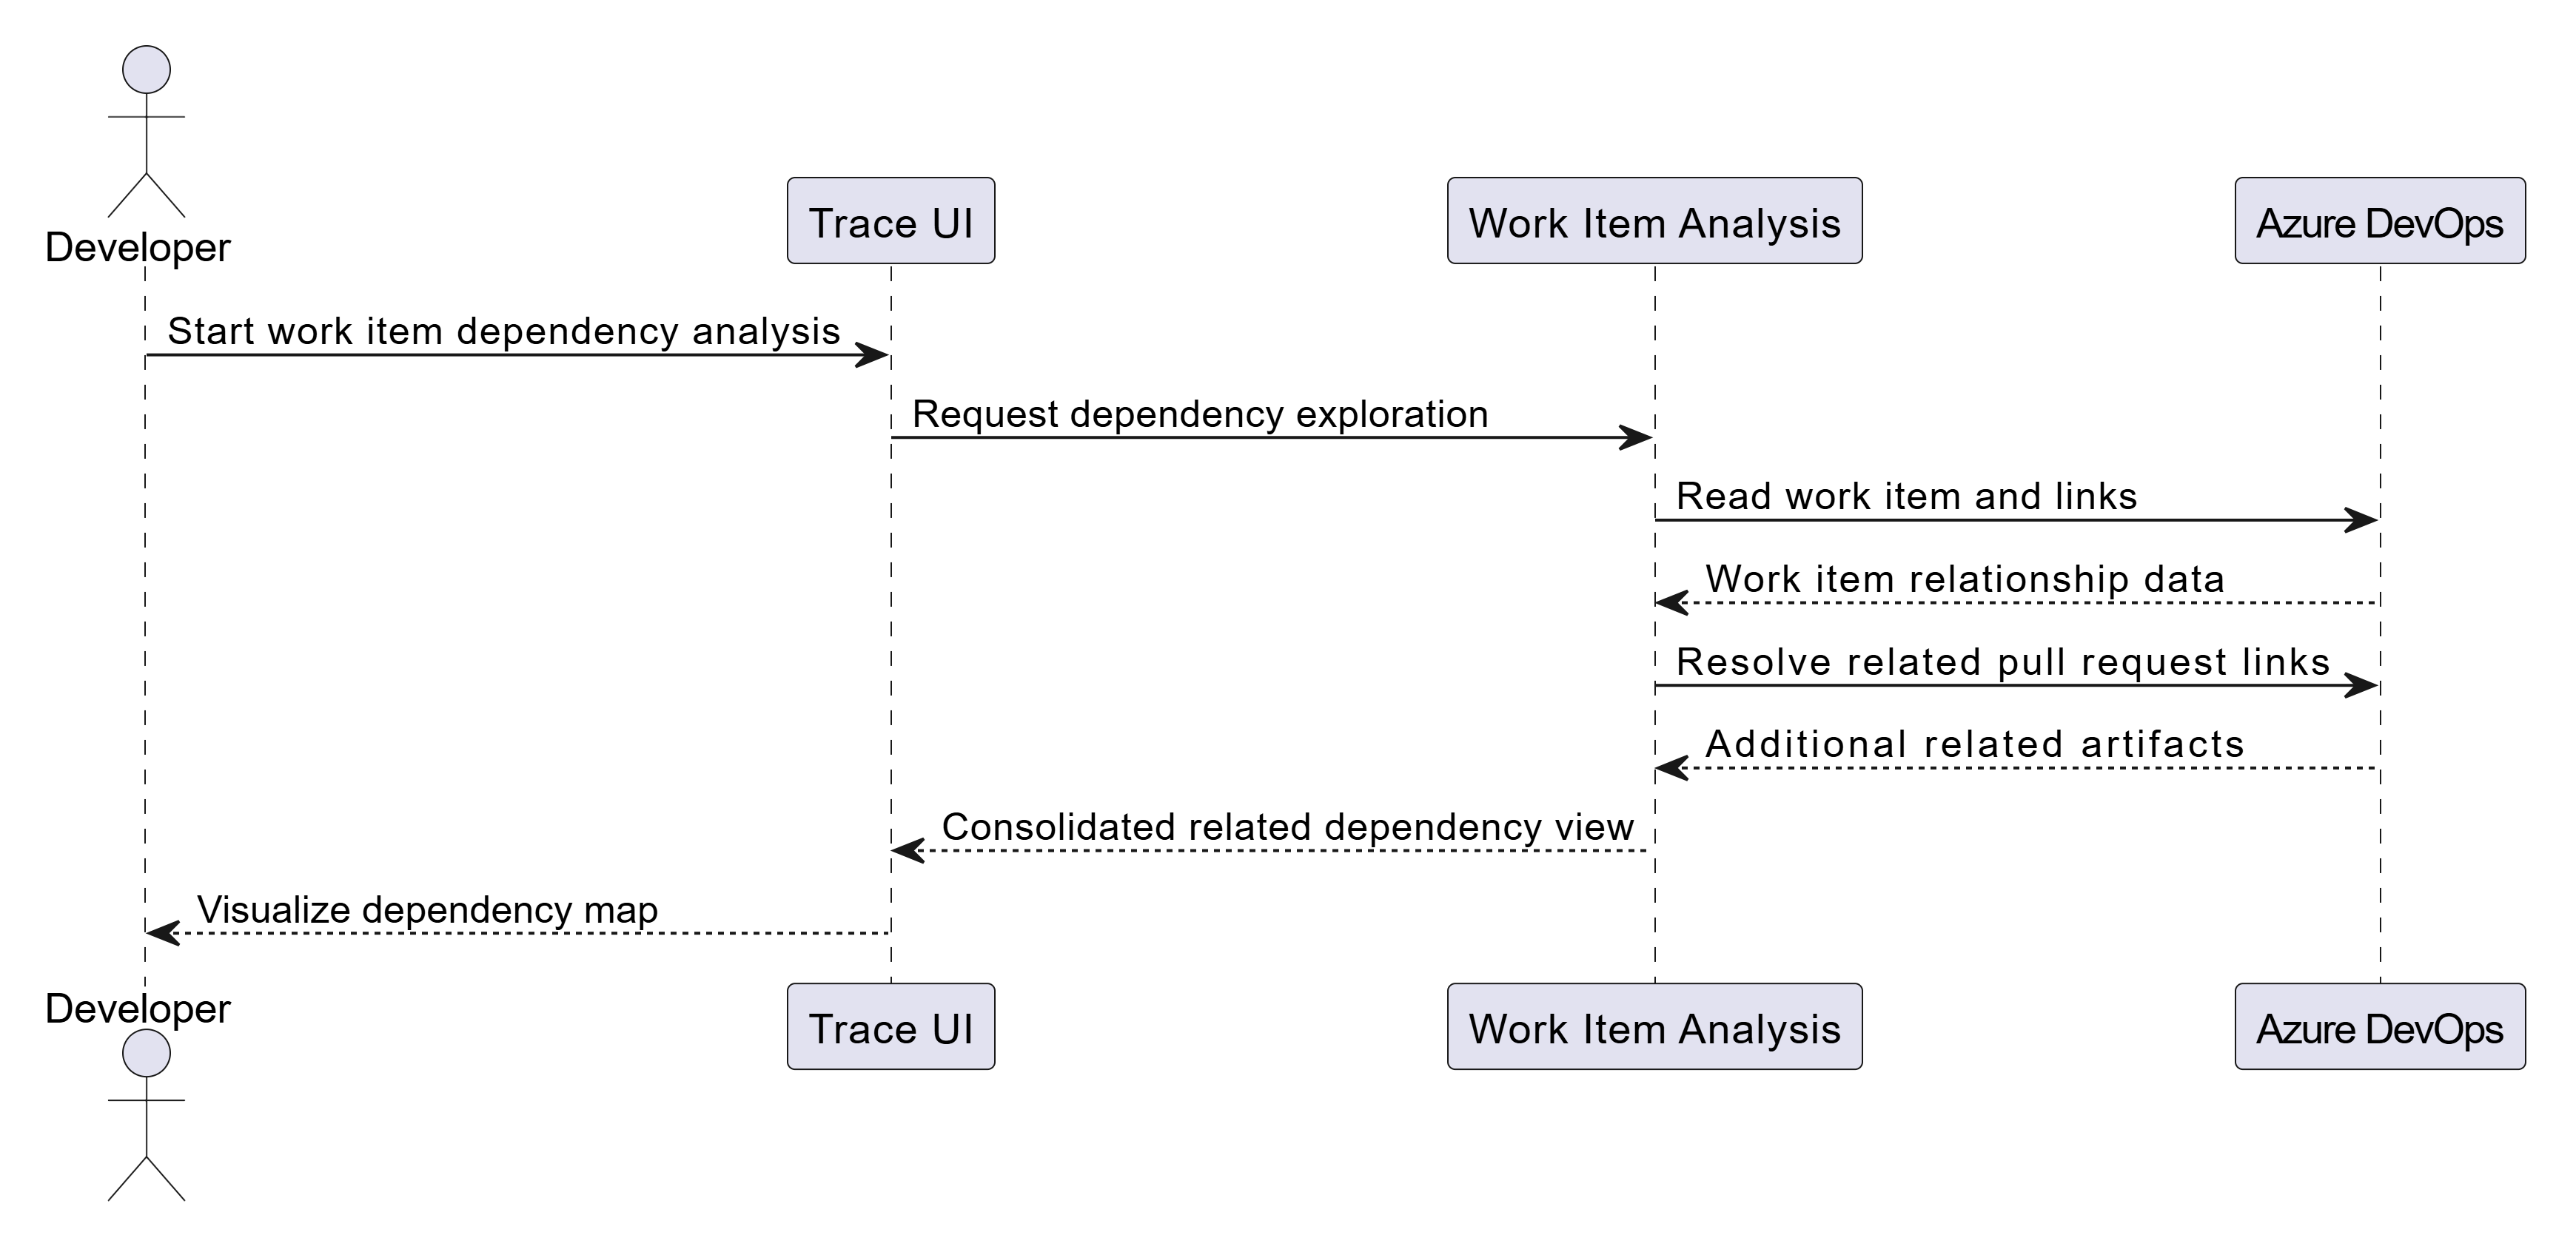
\includegraphics[width=\linewidth]{img/archi/workitemsequence.png}
  \caption{Sequence diagram — Work Item Management Component.}
  \label{fig:workitem-sequence}
\end{figure}

% ─────────────────────────────────────────────────────────────────────────────
\subsection{Pull Request Resolution Component}
\label{subsec:pr-component}

\subsubsection{Role and Responsibility}

The Pull Request Resolution Component bridges the work tracking domain and the
source control domain. Its function is to receive the pull request identifiers
extracted by the Work Item Management Component and resolve them into enriched,
normalized structures that carry both pull request metadata and the identities
of the repositories involved.

This bridging role is architecturally significant. In Azure DevOps, the
connection between a work item and the code changes that implement it passes
through pull requests: a work item links to a pull request, which links to one
or more commits in a specific repository. Without explicit pull request
resolution, the traceability chain would break at the boundary between the work
tracking system and the Git system.

\subsubsection{Pull Request Enrichment Process}

For each pull request identifier received, the component performs the following
operations:

\begin{enumerate}
  \item Query the Azure DevOps Git API for the full pull request metadata,
  including title, status, source branch, target branch, and the identifier of
  the repository in which the PR was created.
  \item Extract the list of work items formally linked to the pull request on
  the Git side — which may differ from the work items that link to the PR on
  the work tracking side.
  \item Construct a normalized \texttt{PullRequestSummaryDto} that exposes the
  PR identifier, the repository name, and the list of associated work item
  references in a stable, contract-conformant form.
\end{enumerate}

\subsubsection{Relationship to Other Components}

The Pull Request Resolution Component serves two consumer roles within the
pipeline. First, it directly enriches the dependency graph produced by the
Work Item Management Component by adding repository-level context to the PR
references identified during traversal. Second, it acts as a prerequisite for
the Commit Aggregation Component: resolving commits requires knowing which
repositories are involved, and this information is produced by pull request
resolution.

\subsubsection{Exposed API Surface}

\begin{itemize}
  \item \texttt{GET /pullrequests/:prId/workitems} — Resolves a pull request
  by its identifier and returns the normalized PR summary together with the
  work items formally linked to it on the Git side.
\end{itemize}

\begin{figure}[htbp]
  \centering
  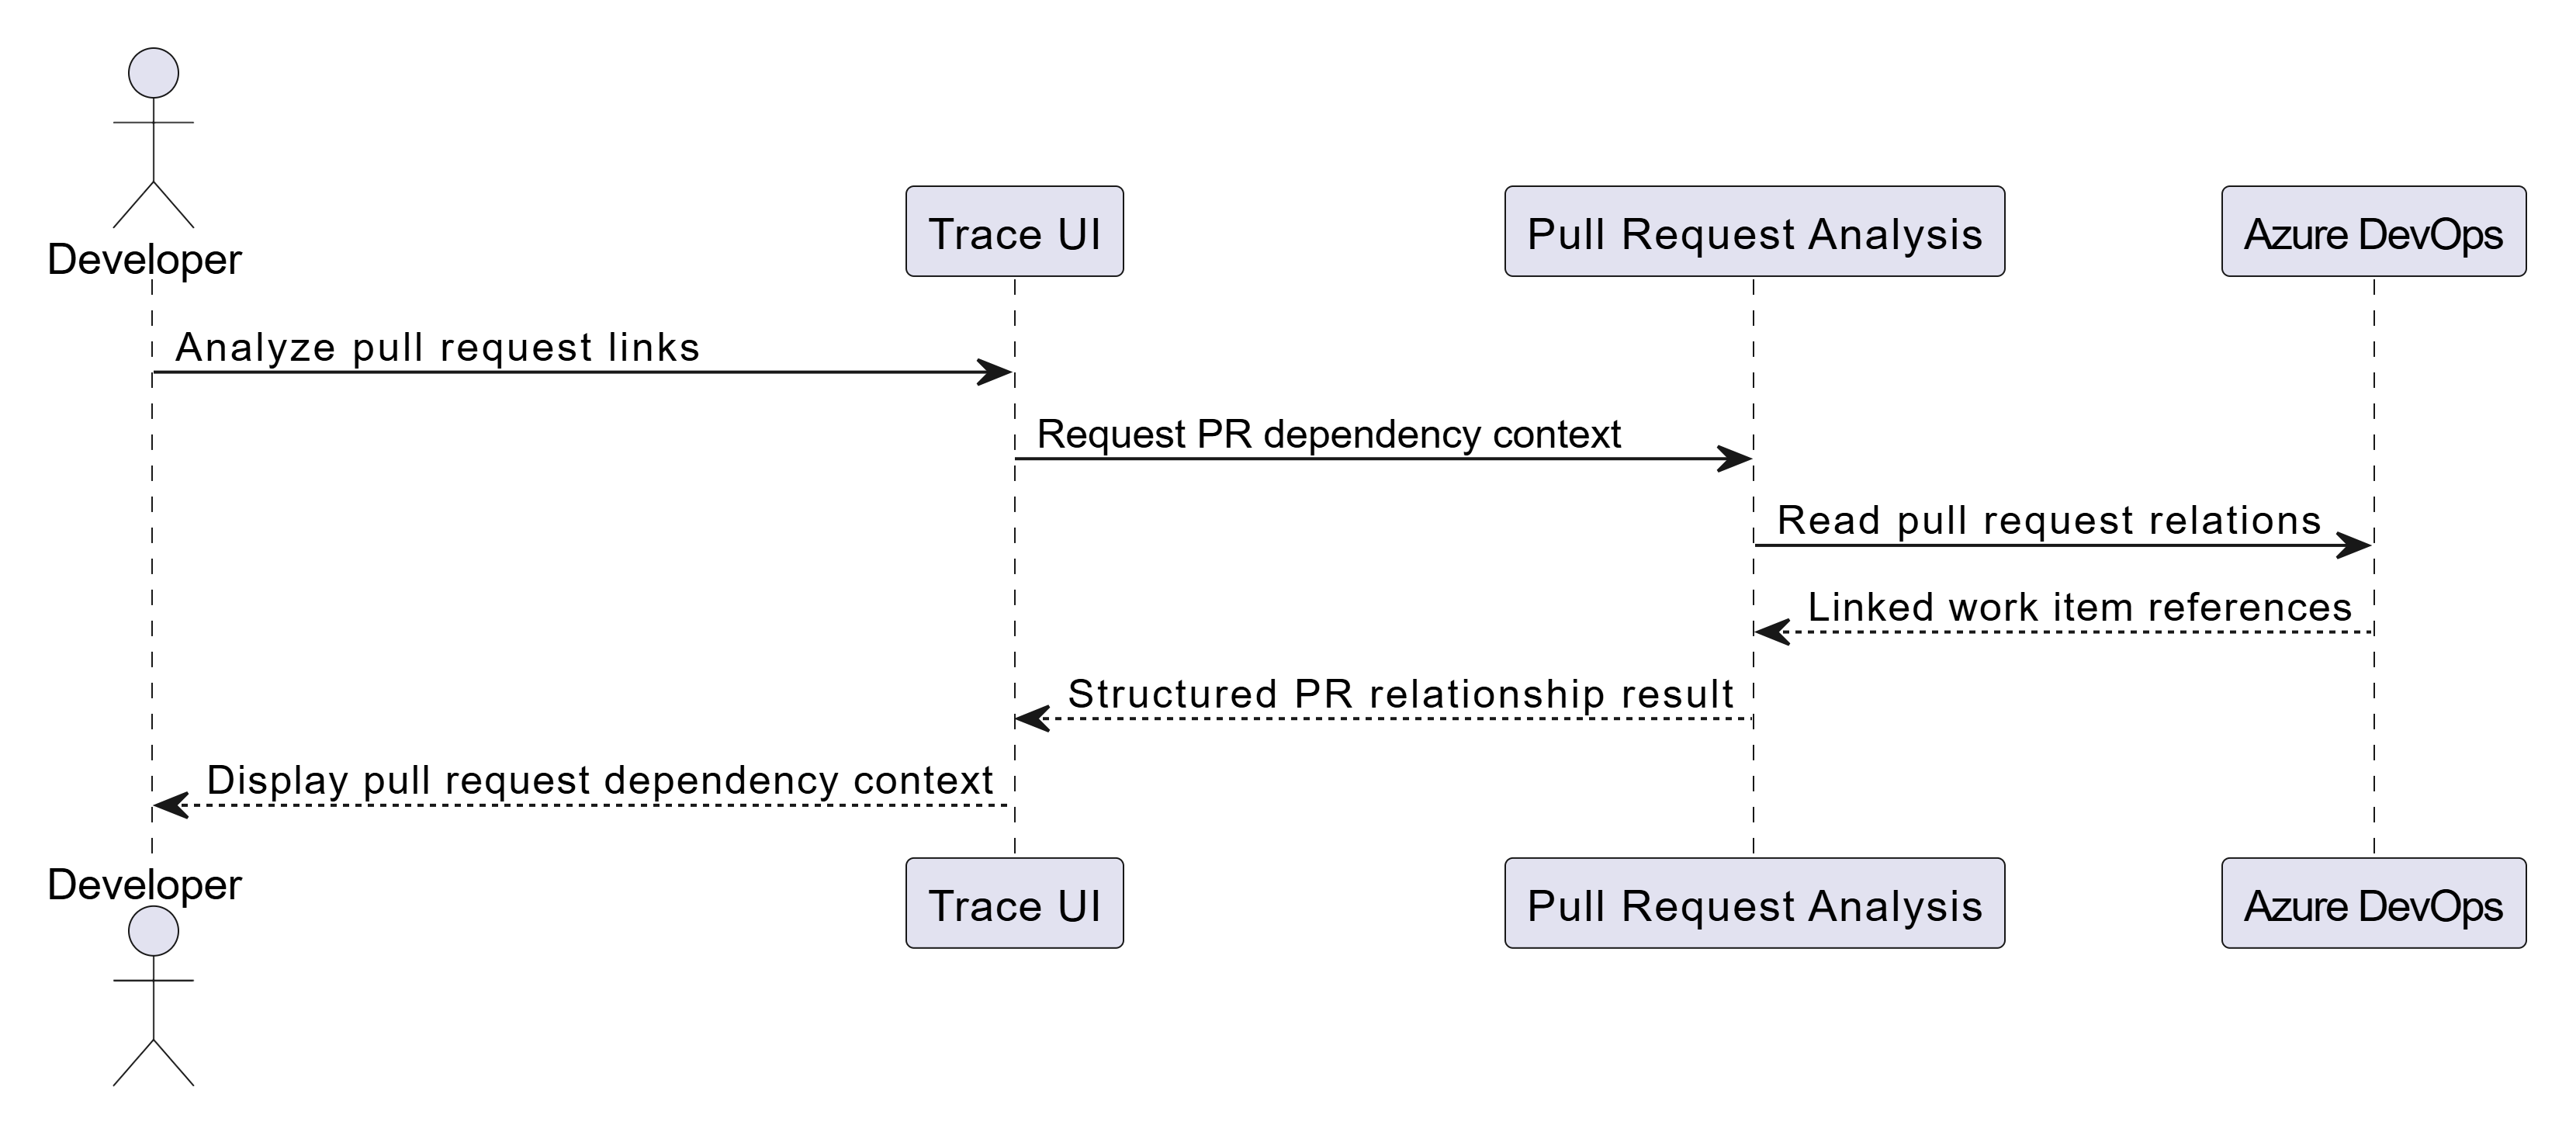
\includegraphics[width=\linewidth]{img/archi/pullrequest.png}
  \caption{Sequence diagram — Pull Request Resolution Component.}
  \label{fig:pullrequest-sequence}
\end{figure}

% ─────────────────────────────────────────────────────────────────────────────
\subsection{Commit Aggregation Component}
\label{subsec:commit-component}

\subsubsection{Role and Responsibility}

The Commit Aggregation Component delivers the finest level of traceability in
the system: it connects work items and pull requests to the actual code changes
that implement them, and it enriches those code changes with the repository
context — branches and tags — needed to determine their position relative to
software releases.

This component answers a critical question that no other layer of the system
addresses: for a given work item or pull request, which commits exist in which
repositories, and what is their release context?

\subsubsection{Commit Resolution Strategy}

The component resolves commits through two complementary mechanisms:

\begin{itemize}
  \item \textbf{Commit resolution via pull request}: The Azure DevOps Git API
  provides the list of commits that were merged as part of a specific pull
  request. This is the primary and most reliable mechanism for establishing
  the work-item-to-commit link when a pull request is present.
  \item \textbf{Commit resolution via work item}: For work items that carry
  direct commit references in their relation metadata, the component resolves
  those references directly through the Work Item Tracking API. This mechanism
  handles scenarios where commits are linked without a formal pull request.
\end{itemize}

In both cases, the resolved commits are deduplicated by commit identifier before
being passed downstream, ensuring that commits referenced through multiple paths
— which is common in complex branching strategies — appear only once in the
result.

\subsubsection{Repository Context Enrichment}

Resolving the commit list is not sufficient for release analysis. Each commit
must also be placed in its repository context: which branches contain it, and
which tags are associated with it. This context is critical for the Decision
Aggregation Component to determine whether a commit falls before or after a
specific release tag.

The component retrieves this context through the Azure DevOps Git API, querying
branch and tag references for each resolved commit. To avoid the prohibitive
cost of issuing one API call per commit, the component applies the
batch-oriented processing principle: it groups commit identifiers by repository
and resolves tag context in a single batched request per repository group.

The tag resolution strategy uses a \emph{latest-tag branch strategy}: for each
commit, the component identifies the most recent tag reachable from the commit
on the relevant branch, providing a meaningful release reference even when a
commit is not directly tagged.

\subsubsection{Internal Service Decomposition}

To maintain clarity and testability, the commit resolution logic is distributed
across four specialized internal services rather than concentrated in a single
large service class:

\begin{itemize}
  \item \textbf{CommitPRService}: resolves commits associated with a specific
  pull request via the Git API.
  \item \textbf{CommitWorkItemService}: resolves commits directly linked to a
  specific work item via the Work Item Tracking API.
  \item \textbf{CommitHistoryService}: queries commit history, branch
  references, and tag references for specific commits and repositories.
  \item \textbf{Utility services}: provide tag selection logic, batch reference
  resolution, and commit deduplication shared across the other services.
\end{itemize}

\subsubsection{Exposed API Surface}

\begin{itemize}
  \item \texttt{GET /commits/workitems/:workItemId} — Returns the deduplicated
  list of commits linked to the specified work item, resolved through both
  direct links and PR expansion.
  \item \texttt{GET /commits/pullrequests/:prId} — Returns the commits
  associated with the specified pull request.
  \item \texttt{GET /commits/branches} — Lists branch and tag names for a
  specified repository.
  \item \texttt{GET /commits/tags} — Resolves branch and tag references
  associated with a specific commit hash.
  \item \texttt{GET /commits/tags/batch} — Batch-resolves tag context for
  multiple commits across one or more repositories in a single request.
\end{itemize}

\begin{figure}[htbp]
  \centering
  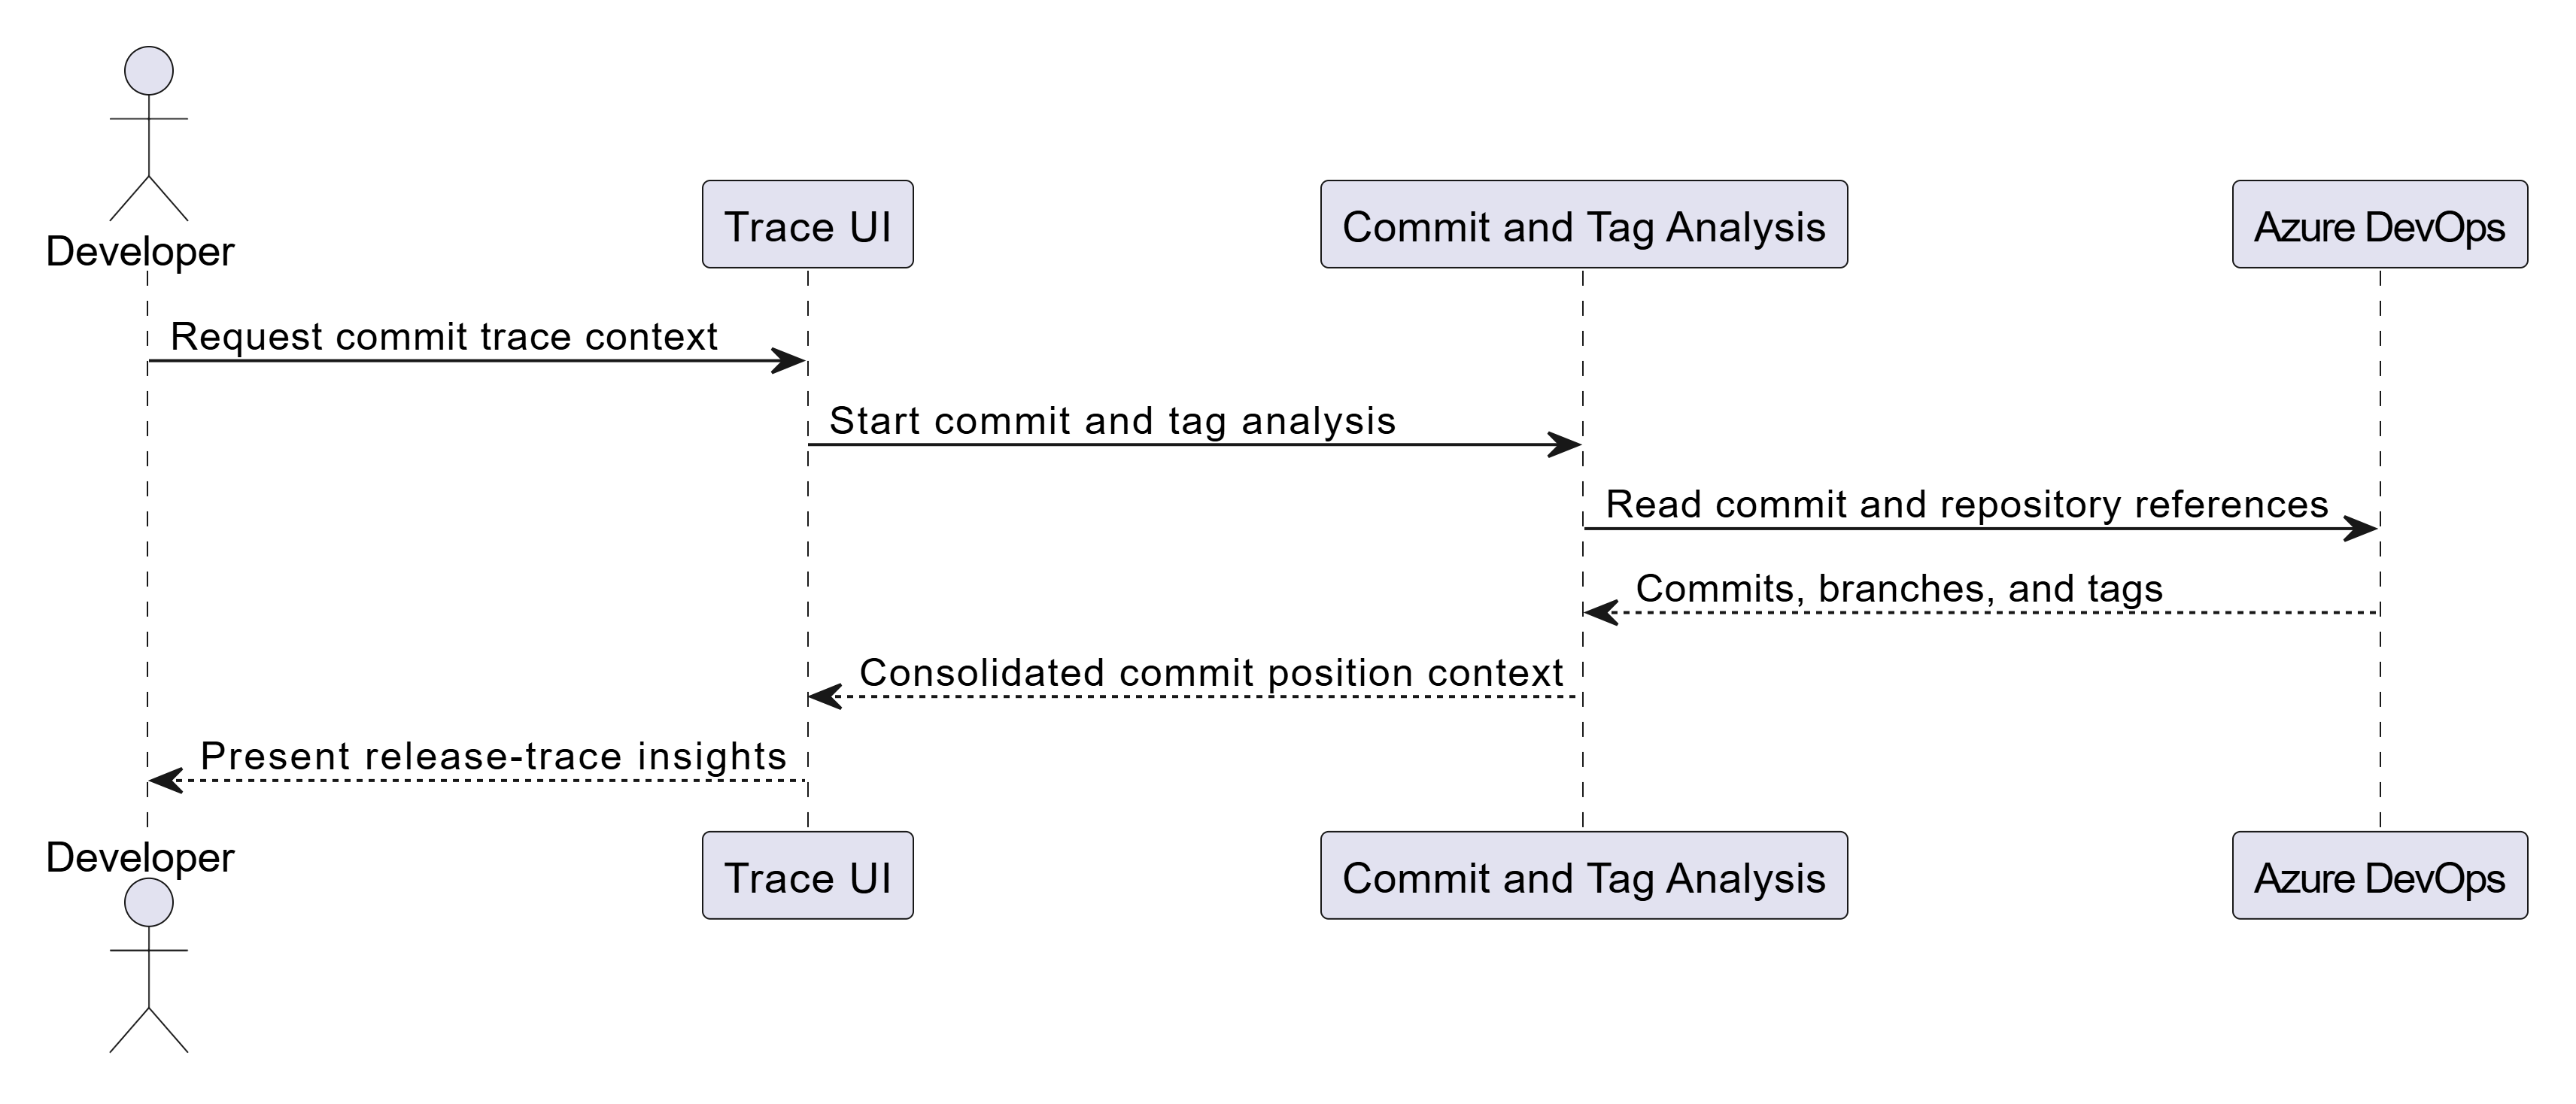
\includegraphics[width=\linewidth]{img/archi/commit.png}
  \caption{Sequence diagram — Commit Aggregation Component.}
  \label{fig:commit-sequence}
\end{figure}

% ─────────────────────────────────────────────────────────────────────────────
\subsection{Decision Aggregation Component}
\label{subsec:decision-component}

\subsubsection{Role and Responsibility}

The Decision Aggregation Component represents the final analytical stage of the
traceability pipeline. Unlike the three preceding components, it does not issue
any queries to Azure DevOps. Instead, it operates entirely on the normalized
data produced and collected by the upstream components, applying a classification
logic that transforms raw trace data into a structured, decision-ready output.

The central question this component addresses is: \emph{given the full set of
work items and their associated commits, what is the release readiness status
of each repository involved in the dependency graph?}

\subsubsection{Classification Logic}

The component receives a consolidated trace payload — containing work items with
their states, pull request summaries, and per-repository commit lists with tag
context — and applies a multi-step classification process:

\begin{enumerate}
  \item \textbf{Work item status partitioning}: work items are divided into two
  groups based on their current Azure DevOps state — those whose state maps to
  a \emph{done} condition (e.g., Closed, Resolved, Done) and those whose state
  indicates remaining work (e.g., Active, In Progress, New). This partition
  establishes whether the functional requirements carried by the work items have
  been fully delivered.

  \item \textbf{Repository commit classification}: for each repository present
  in the commit trace, the component examines the tag context of the associated
  commits and classifies the repository into one of three release-relative
  buckets:
  \begin{itemize}
    \item \textbf{Before-and-after}: the repository contains commits both before
    and after the reference tag, indicating that changes straddle a release
    boundary.
    \item \textbf{Only-before}: all commits in the repository predate the
    reference tag, indicating that the changes were fully included in the
    referenced release.
    \item \textbf{Only-after}: all commits in the repository postdate the
    reference tag, indicating that the changes are part of a future release
    scope.
  \end{itemize}

  \item \textbf{Pull request relevance marking}: when a commit should be
  highlighted for pull request integration, the component sets a dedicated
  \texttt{considerForPR} flag in the output. This makes the recommendation
  explicit without forcing the user to infer it from raw tag data.
\end{enumerate}

\subsubsection{Stateless and Deterministic Design}

A key design property of this component is that it is entirely stateless and
deterministic. Given the same input trace payload, it will always produce the
same classification output. This property makes the component straightforward
to test, easy to reason about, and safe to invoke multiple times without side
effects.

The stateless design also means that the component can be invoked independently
of the rest of the pipeline — for example, to recompute a decision view when
the user changes the reference tag — without needing to repeat the upstream
data collection steps.

\subsubsection{Exposed API Surface}

\begin{itemize}
  \item \texttt{POST /decision/aggregate} — Accepts a structured trace payload
  and returns the classified decision output, including the work item status
  partition, per-repository decision buckets, and commit-level PR relevance
  flags.
\end{itemize}

\begin{figure}[htbp]
  \centering
  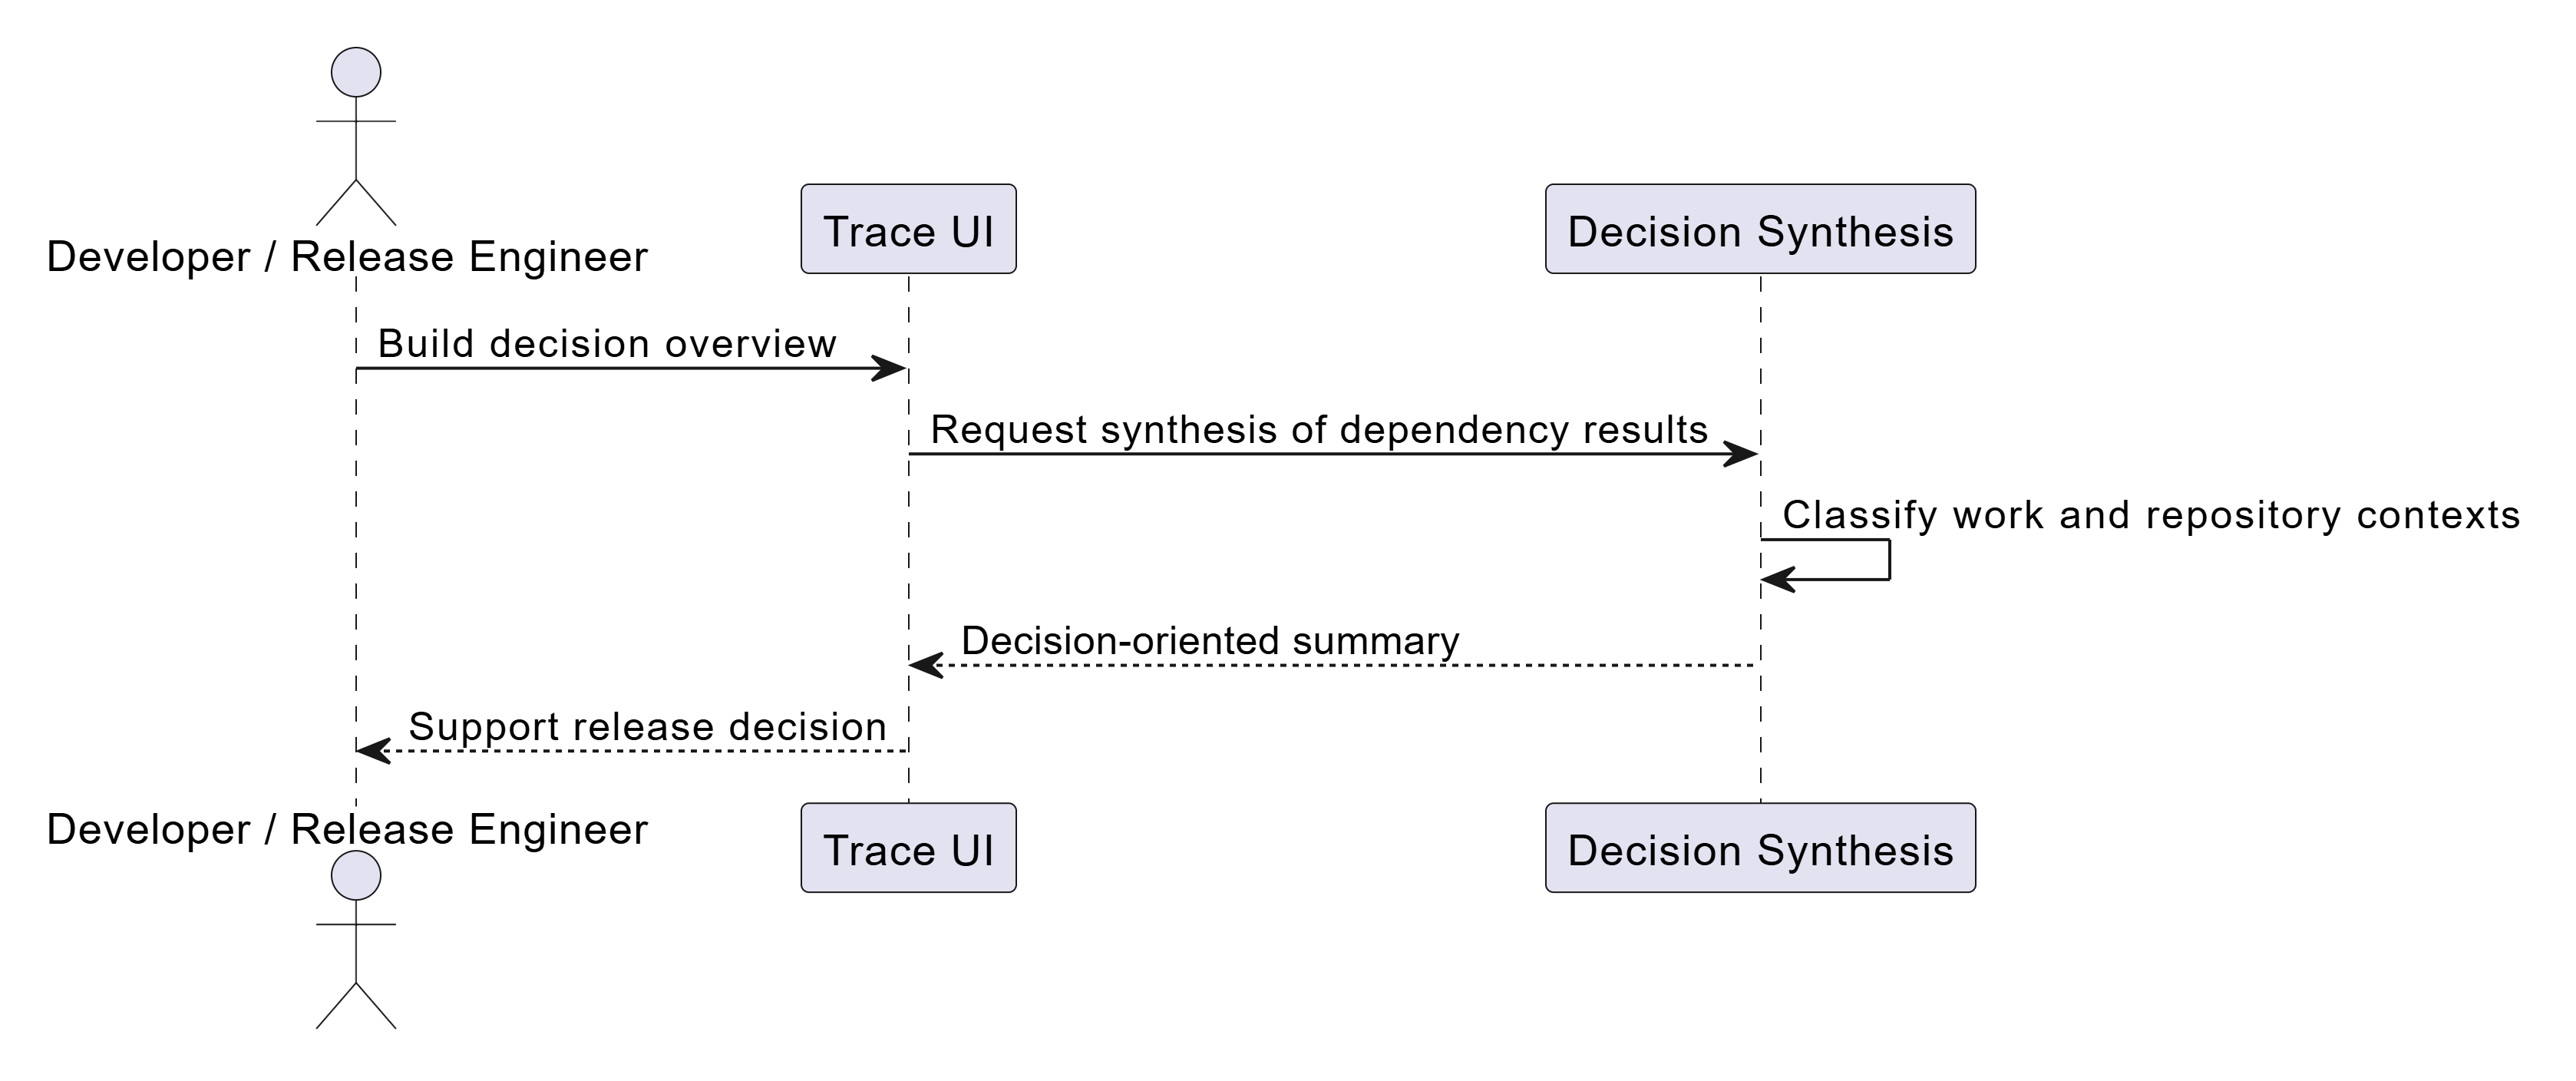
\includegraphics[width=\linewidth]{img/archi/decision.png}
  \caption{Sequence diagram — Decision Aggregation Component.}
  \label{fig:decision-sequence}
\end{figure}


% ─────────────────────────────────────────────────────────────────────────────
\section{Data Contracts and Normalization Model}
\label{sec:data-contracts}

A critical structural element of the proposed solution is its systematic use of
Data Transfer Objects (DTOs) as the exclusive mechanism for data exchange across
module boundaries, API surfaces, and layer transitions. This section describes
the data contract model and the normalization strategy that underlies it.

\subsection{Role of Data Transfer Objects}

DTOs serve two distinct but complementary roles in the system. At the
\textbf{input} boundary, they enforce the structure and validity of data
entering a module — whether from the Presentation Layer or from an upstream
pipeline stage. At the \textbf{output} boundary, they define the stable,
documented shape of data that a module guarantees to its consumers.

This dual role means that every data transformation in the system is explicit
and traceable. When a developer reads the output DTO of a module, they have a
complete and accurate description of what that module produces — not an implicit
understanding derived from reading implementation code.

\subsection{Main Data Contract Groups}

The system defines five primary groups of data contracts:

\begin{itemize}
  \item \textbf{Work Item Contracts}: \texttt{WorkItemDto} represents one
  normalized work item with its identifier, title, type, state, assignee, and
  typed relation links through \texttt{WorkItemLinkDto}. Single-root traversal
  results are wrapped in \texttt{RelatedWorkItemsDataDto}, while multi-root
  traversals use \texttt{RelatedWorkItemsBatchDataDto}.

  \item \textbf{Pull Request Contracts}: \texttt{PullRequestSummaryDto}
  provides a lightweight normalized representation of a pull request within the
  traceability context, exposing the PR identifier and the repository name. This
  DTO is embedded in both work item trace responses and pull request module
  responses, creating a consistent cross-module reference.

  \item \textbf{Commit and Repository Contracts}: \texttt{CommitInfo} carries
  the commit identifier and repository name as a minimal reference embedded in
  trace responses. Richer DTOs — \texttt{CommitsByWorkItemResponseDto},
  \texttt{CommitsByPRResponseDto}, \texttt{RepoReferencesResponseDto} — provide
  full commit lists with branch and tag context for consuming components.

  \item \textbf{Streaming Event Contracts}: SSE messages carry structured
  payloads defined by dedicated event DTOs. Batch progress messages expose the
  batch content, the batch sequence number, and the cumulative count of resolved
  items. Completion and error messages follow distinct schemas to allow the
  consumer to unambiguously identify the event type.

  \item \textbf{Decision Contracts}: the input payload of the final
  classification stage is described by \texttt{DecisionAggregateInputDto}, and
  the output is described by \texttt{DecisionAggregateOutputDto}. Together,
  they define the work item status groups, repository-level decision buckets,
  and commit-level pull request relevance flags returned by the system.
\end{itemize}

\subsection{Normalization at the Integration Boundary}

All normalization from raw Azure DevOps API responses to internal DTOs occurs
at the Integration Layer boundary, within shared utility functions dedicated to
this transformation. These utilities handle the structural parsing of Azure
DevOps relation types, the extraction of embedded identifiers (such as pull
request IDs encoded in work item relation URLs), and the mapping of Azure
DevOps field names to the internal model.

This boundary normalization ensures that no module ever encounters raw Azure
DevOps response data in its processing logic. All processing, classification,
and enrichment operates on a clean, homogeneous internal model.


% ─────────────────────────────────────────────────────────────────────────────
\section{End-to-End Data Flow}
\label{sec:data-flow}

The four core components operate together in a clear, sequential pipeline that
connects user intent to actionable analytical output. This section traces the
complete execution path of an analysis session, illustrating how each component
contributes to the progressive enrichment of the dependency graph.

\begin{figure}[htbp]
  \centering
  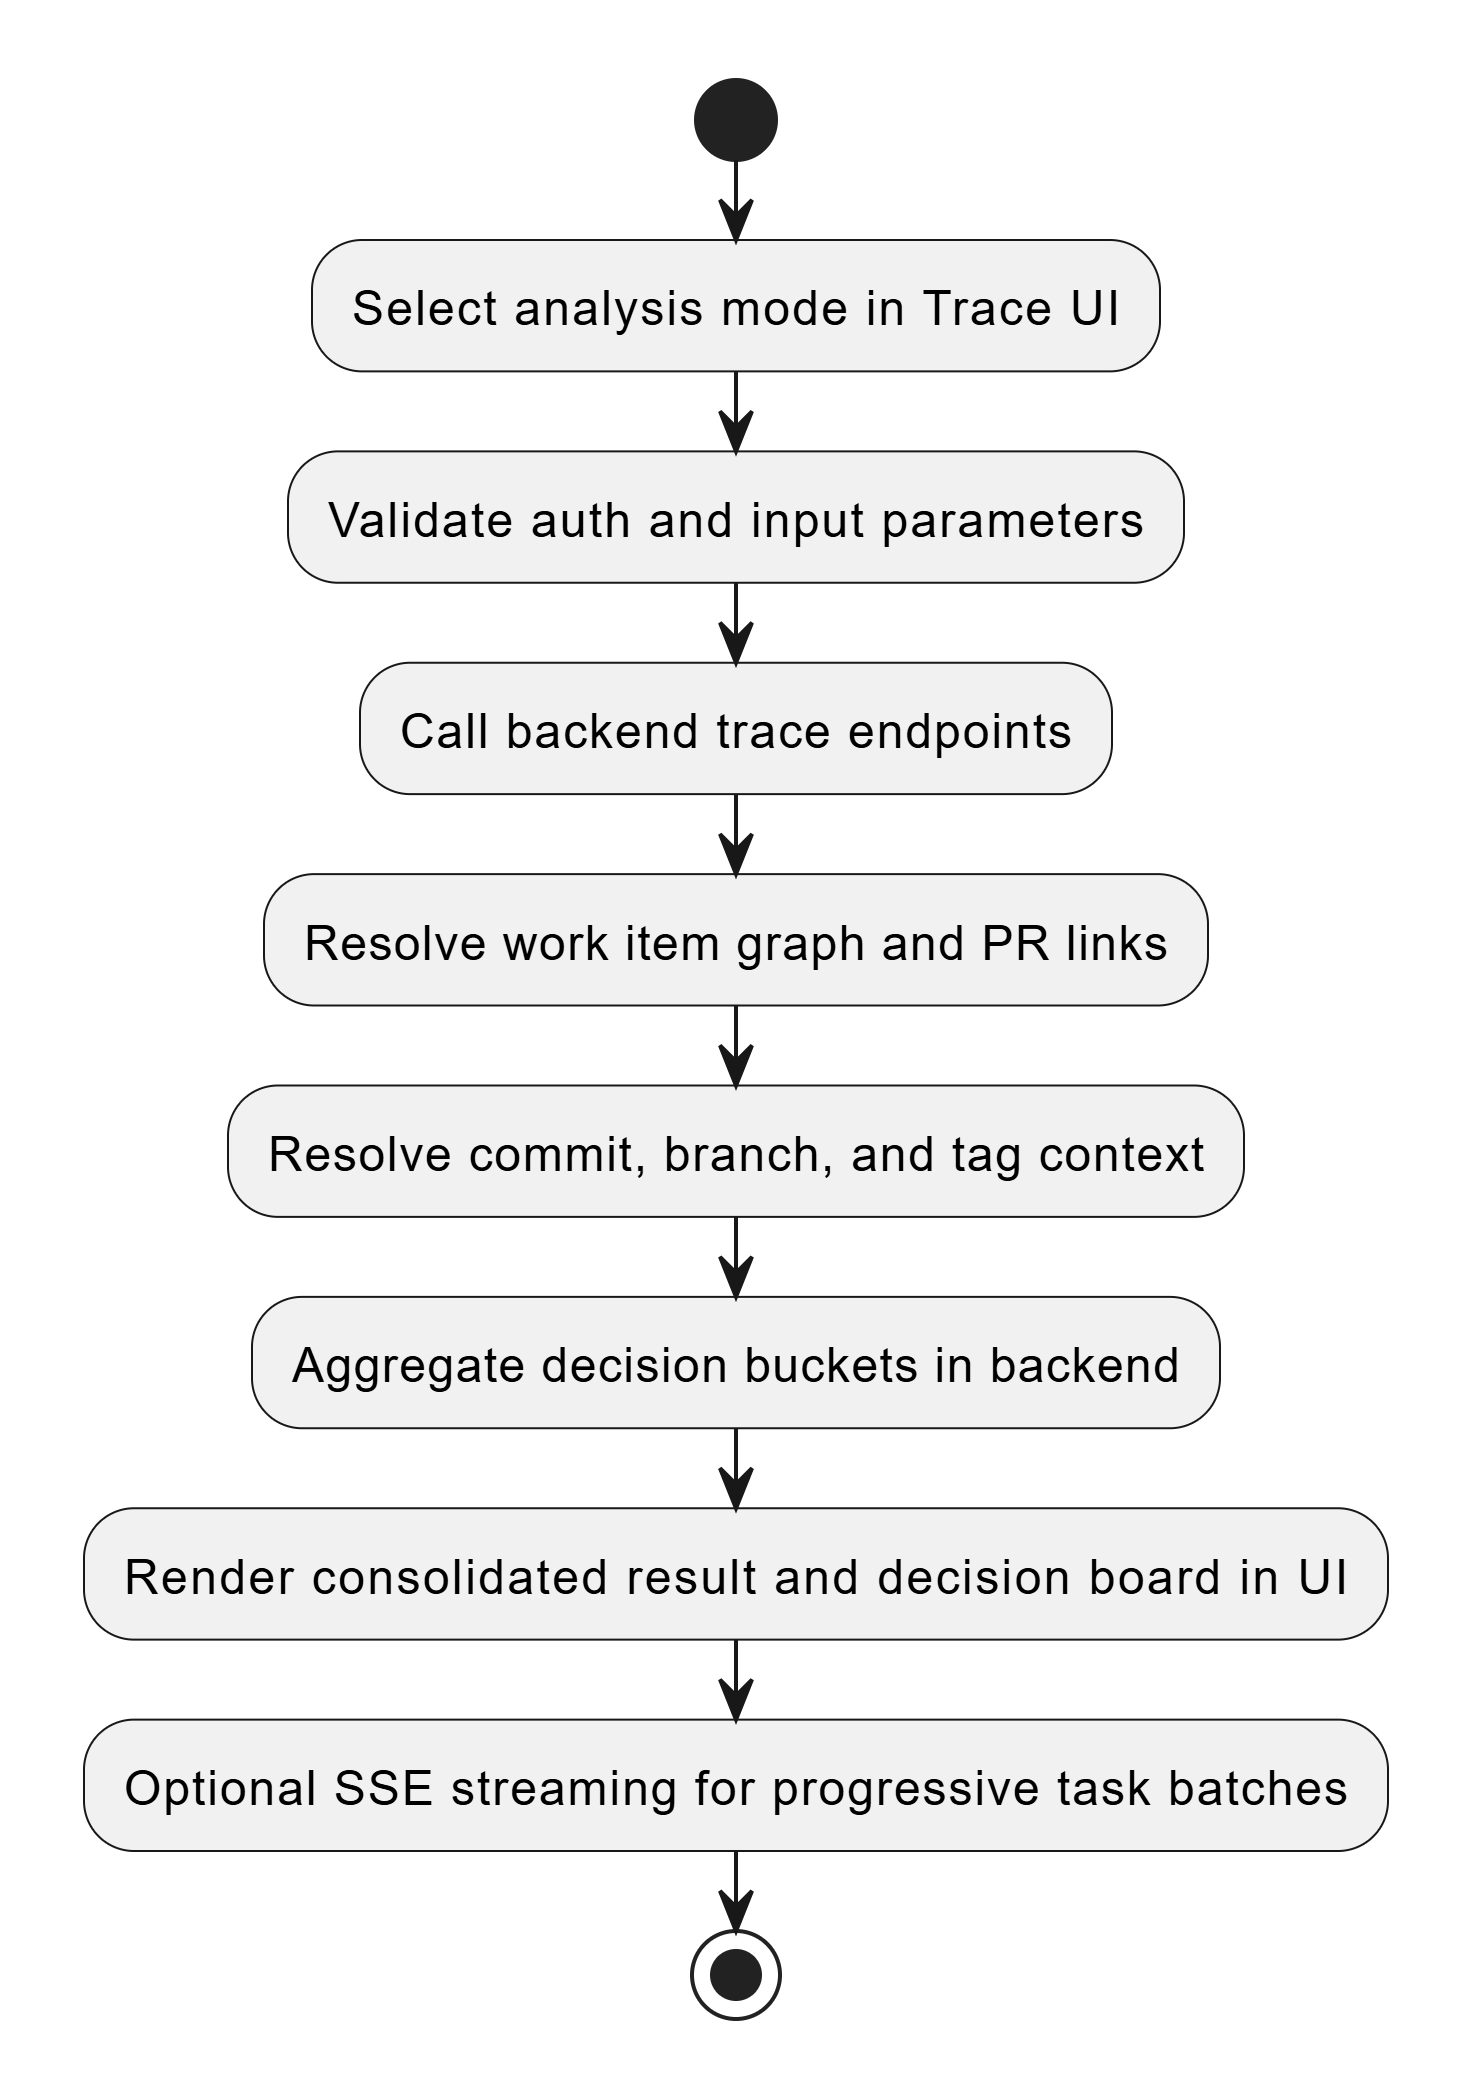
\includegraphics[width=\linewidth]{img/archi/end_end.png}
  \caption{End-to-end data flow across the four system components.}
  \label{fig:end-to-end-flow}
\end{figure}

\subsection{Step 1 — User Initiates the Analysis}

The user accesses the Trace UI and selects an analysis mode. In single-trace
mode, the user provides a single work item identifier. In batch mode, the user
selects multiple work items from a streamed task list. In batch-related mode,
the user triggers an aggregated analysis across all selected roots simultaneously.

The UI validates the user input and constructs a well-formed request that
includes the work item identifiers, the Azure DevOps project context, and any
additional parameters such as the analysis depth or the reference tag for
decision classification.

\subsection{Step 2 — Work Item Graph Construction}

The request reaches the backend, where the Work Item Management Component begins
the dependency graph traversal. It retrieves the specified root work items from
the Azure DevOps Work Item Tracking API and expands the graph level by level,
following parent/child and related-item links. Visited states are tracked to
prevent cycles. Items are retrieved in batches, and results are cached to avoid
redundant calls.

At the end of this stage, the component has produced:
\begin{itemize}
  \item a complete, normalized list of all work items reachable from the
  specified roots;
  \item a deduplicated list of pull request identifiers extracted from the
  relation metadata of visited work items.
\end{itemize}

\subsection{Step 3 — Pull Request Resolution and Repository Identification}

The Pull Request Resolution Component receives the list of pull request
identifiers produced in the previous stage. For each identifier, it queries the
Azure DevOps Git API to retrieve the PR metadata and the list of work items
formally linked to the PR on the Git side. It constructs a normalized
\texttt{PullRequestSummaryDto} for each PR, capturing the repository name
alongside the PR identifier.

At the end of this stage, the dependency graph has been enriched with:
\begin{itemize}
  \item normalized pull request summaries associated with the relevant work
  items;
  \item the repository identities of all repositories involved in the analysis.
\end{itemize}

\subsection{Step 4 — Commit Resolution and Repository Context Enrichment}

The Commit Aggregation Component uses the pull request summaries and repository
identifiers produced in the previous stage to resolve commits. For each pull
request, it queries the Git API to retrieve the list of commits merged as part
of that PR. For work items with direct commit links, it resolves those commits
independently.

All resolved commits are deduplicated and grouped by repository. The component
then performs batch tag resolution: for each repository group, it issues a
single API request to resolve the branch and tag context of all relevant commits
simultaneously.

At the end of this stage, the dependency graph is complete in the sense that
every artifact in the traceability chain — from work item to commit — is
represented, normalized, and enriched with release context.

\subsection{Step 5 — Decision Classification}

The Decision Aggregation Component receives the fully enriched trace payload
and applies its classification logic. Work items are partitioned by completion
state. Repositories are classified into release-relative decision buckets based
on the tag context of their associated commits. Commits of particular relevance
for pull request integration are flagged accordingly.

The output is a structured decision payload that directly answers the
release-readiness question: which repositories are fully integrated, which
straddle a release boundary, and which remain outside the current release scope.

\subsection{Step 6 — Result Delivery and Visualization}

The classified decision payload, together with the full trace data, is returned
to the Trace UI. The UI assembles the final view state and renders the results
across its specialized view components: the dependency graph view for work item
hierarchies, the repository grouping view for commit-level context, and the
Decision Dashboard for release classification output.

The user can interact with the results, drill down into specific work items or
repositories, and use the Decision Dashboard output to inform release, integration,
and escalation decisions.


% ─────────────────────────────────────────────────────────────────────────────
\section{User Interface Design and Interaction Model}
\label{sec:ui-design}

Although the backend performs the core analysis, the value of the system also
depends on how clearly the results are exposed to end users. This section
summarizes the three analysis modes supported by the Trace UI and explains the
type of user interaction expected in each case.

\subsection{Single Work Item Trace Mode}

In this mode, the user enters one work item identifier and launches a focused
analysis. The system traverses the dependency graph rooted at that item,
resolves the related pull requests and commits, and presents the result in a
structured view. This mode is well suited to targeted impact analysis, for
example when verifying the implementation scope of a specific user story.

\subsection{Batch Work Item Trace Mode}

In batch mode, the user receives a progressively loaded list of available work
items through the SSE endpoint, selects several of them, and then launches a
group analysis. This mode is useful when preparing a release or reviewing a
sprint scope, because it reveals all repositories and commits involved in the
selected set.

\subsection{Batch-Related Work Item Trace Mode}

This mode performs a parallel dependency analysis across all selected roots and
then consolidates the result. The work items can be ranked by the breadth of
their dependency footprint, and the Decision Dashboard is displayed to support
release-oriented interpretation of the aggregated result.

\subsection{Observability and Progress Feedback}

One important design objective of the Trace UI is to keep users informed during
long-running analyses. Thanks to streaming, results appear progressively instead
of after one long blocking delay. The interface also exposes the SSE connection
state --- connecting, open, reconnecting, or closed --- so that users can
understand what the system is doing at each stage of the analysis.


% ─────────────────────────────────────────────────────────────────────────────
\section{Operational Observability and Logging Strategy}
\label{sec:observability}

Operational observability is treated as a first-class system property, not an
afterthought. The system implements a structured logging strategy using the
\textbf{AppLogger} framework, applied consistently across all backend modules
and service layers.

\subsection{Log Level Strategy}

Different log levels are used strategically across the pipeline to maintain a
clean operational signal while preserving diagnostic depth when needed:

\begin{itemize}
  \item \texttt{log}: normal operation events — component invocations,
  traversal progress, batch boundaries, and successful API call completions.
  These form the standard operational trace of a healthy analysis session.
  \item \texttt{warn}: recoverable anomalies — partial data returns, unexpected
  API response shapes, rate limit proximity signals, and items skipped due to
  missing relations. These do not interrupt processing but indicate conditions
  worth monitoring.
  \item \texttt{error}: failures requiring attention — API call failures after
  retry exhaustion, data normalization failures, and unresolvable dependency
  links. These are logged with full context to support root cause analysis.
  \item \texttt{debug} and \texttt{verbose}: detailed diagnostic output —
  individual work item relation resolution, cache hit/miss events, batch
  composition details, and tag resolution results. These are intended for
  development and troubleshooting and are suppressed in normal operation.
\end{itemize}

\subsection{Observability Value in a Traceability System}

Structured logging is especially valuable in a system that depends on external
APIs for correctness. When an analysis produces unexpected results — a missing
commit, an incomplete graph, or an incorrect decision classification — structured
logs allow the developer or operator to reconstruct the exact sequence of API
calls and data transformations that led to the output, without requiring a
debugger or a reproduction environment.

The logging strategy also provides an audit trail for analysis sessions, which
can be used to verify that a specific analysis was performed correctly and to
compare results across successive sessions.


% ─────────────────────────────────────────────────────────────────────────────
\section{System Advantages}
\label{sec:advantages}

The proposed solution delivers concrete advantages over the current state of
practice, addressing both the functional gaps identified in the problem analysis
and broader non-functional requirements of reliability, scalability, and
maintainability.

\subsection{Centralized and Unified Visibility}

The most immediate advantage of the solution is the consolidation of scattered
dependency information into a single, coherent analytical interface. Before this
system, understanding the full dependency chain of a work item required a
developer or release engineer to navigate across multiple Azure DevOps views —
the work item board, the pull request list, the repository commit history, and
the branch/tag management interface — and manually correlate the information
found in each.

The proposed system eliminates this manual correlation step. A single analysis
session retrieves, normalizes, enriches, and presents the complete dependency
chain from work item to commit, in a structured format that supports immediate
decision-making.

\subsection{Improved Release Decision Support}

The Decision Aggregation Component translates raw trace data into a structured
release classification that directly answers the questions relevant to a release
decision: which repositories are fully integrated, which straddle the release
boundary, and which changes fall outside the current scope. This structured
output reduces the time required to assess release readiness and reduces the
risk of releasing incomplete or incorrectly integrated changes.

\subsection{Scalability for Large Projects}

The batch-oriented processing strategy, combined with in-memory caching and
SSE-based progressive delivery, makes the system viable for large projects with
deep dependency graphs. Analysis sessions involving dozens of root work items,
hundreds of related items, and thousands of commits across multiple repositories
can be completed efficiently and presented to the user with real-time progress
feedback — a use case that is practically infeasible with manual Azure DevOps
navigation.

\subsection{Consistency and Reliability of Results}

The systematic normalization of all Azure DevOps API responses at the integration
boundary ensures that analysis results are consistent and reliable regardless of
the structural variations present in the underlying data. Users can trust that
the same query will produce the same result across successive sessions, and that
changes in Azure DevOps API response structure will be absorbed at the
normalization layer without affecting the rest of the pipeline.

\subsection{Extensibility for Future Artifact Types}

The modular architecture of the Application Layer makes it straightforward to
extend the traceability scope beyond the artifact types supported in the current
version. New dependency types — such as pipeline run artifacts, automated test
results, release deployment records, or cross-project work item links — can be
introduced as new modules alongside the existing four, following the same
controller/service/DTO pattern and integrating into the pipeline through
well-defined data contracts. No modification to the existing modules or the core
traversal logic is required.

\subsection{Shared Reference for Cross-Functional Collaboration}

By providing a single, factual, and reproducible view of dependencies, the
system creates a shared reference that can be used consistently across roles.
Developers, release engineers, technical leads, and project managers can all
consult the same analysis output to discuss scope, impact, and readiness —
reducing misalignments that arise from each stakeholder navigating the same data
through different interfaces and arriving at different conclusions.


% ─────────────────────────────────────────────────────────────────────────────
\section{Conclusion}
\label{sec:solution-conclusion}

This chapter has presented the proposed solution for structured dependency
traceability in Azure DevOps environments. The system is designed around a
three-layer architecture, four fundamental design principles, and a sequential
pipeline of four specialized components that together transform user-provided
work item identifiers into a fully classified, decision-ready dependency view.

Several design decisions stand out as particularly significant. The adoption of
a contract-first, DTO-based data model ensures stability and consistency across
all module boundaries. The batch-oriented processing strategy makes the system
viable at scale without overwhelming external APIs. The integration of SSE-based
progressive streaming provides a responsive user experience even during
long-running analysis sessions. And the stateless, deterministic design of the
Decision Aggregation Component makes the classification logic transparent and
easily testable.

Together, these decisions produce a system that is not only functional today but
structured for extension and evolution as the traceability requirements of the
organization grow.

The following chapter details the technical implementation of this architecture:
the technologies, frameworks, and implementation patterns used to realize each
component, and the engineering decisions taken during the development process.
\newpage

%% ── Chapter 5 — Implementation ──────────────────────────────────────────────
% ═══════════════════════════════════════════════════════════════════════════════
\chapter{Implementation}
% ═══════════════════════════════════════════════════════════════════════════════

\section{Introduction}

This chapter covers the technical implementation of the MES-X dependency
traceability system, describing how the proposed architecture was built into a
working full-stack application. The system brings together work items, pull
requests, commits, branches, tags, sprint planning data, and AI-assisted
review into a single coherent workflow.

The chapter starts with the technology stack, then walks through the
development approach, backend modules, frontend integration, deployment setup,
and the quality practices used to validate the final product.

% ──────────────────────────────────────────────────────────────────────────────
\section{Technology Stack and Architecture}

MES-X is built on a modern full-stack architecture designed to handle
large-scale dependency graph reconstruction and traceability analysis
efficiently.

\subsection{Web Application Layer (Frontend)}

The frontend is the main interface operators use to run and explore
traceability analyses. It is built for responsiveness and clarity when
rendering complex dependency graphs.

\textbf{Technical specifications:}
\begin{itemize}
  \item \textbf{Framework:} Vue 3 with TypeScript
  \item \textbf{UI framework:} Quasar component system
  \item \textbf{Build tool:} Vite
  \item \textbf{Purpose:} trace execution, progressive visualization, and dependency navigation
\end{itemize}

\begin{figure}[htbp]
  \centering
  
\includegraphics[width=0.45\linewidth]{img/logo/vuejs.png}
  \caption{Frontend technology used: Vue 3 for building the user interface}
  \label{fig:vue-logo}
\end{figure}

% ──────────────────────────────────────────────────────────────────────────────
\subsection{Backend Service Layer}

The backend is the core of the system. It handles traceability logic and
exposes structured APIs for both single and batch analysis.

\textbf{Technical specifications:}
\begin{itemize}
  \item \textbf{Framework:} NestJS (TypeScript)
  \item \textbf{API styles:} REST for queries, SSE for streaming
  \item \textbf{Role:} orchestrating dependency graph construction
\end{itemize}

The backend is organized into domain-driven services, each responsible for
processing and enriching a specific part of the traceability data.

\begin{figure}[htbp]
  \centering
  
\includegraphics[width=0.45\linewidth]{img/logo/nestjs.png}
  \caption{Backend technology used: NestJS for scalable server-side architecture}
  \label{fig:nestjs-logo}
\end{figure}

% ──────────────────────────────────────────────────────────────────────────────
\subsection{Domain Service Layer}

This layer holds the core business logic of the system:

\begin{itemize}
  \item Work item graph traversal and relationship resolution
  \item Pull request linkage and analysis
  \item Commit extraction and repository context resolution
  \item Sprint-to-work-item retrieval for seeding batch traces
  \item LLM-assisted commit review with project-specific guidance
  \item Tag and branch contextual enrichment
\end{itemize}

\textbf{Key responsibilities:}
\begin{itemize}
  \item dependency graph construction
  \item deduplication and cycle prevention
  \item structured data enrichment for UI consumption
\end{itemize}

% ──────────────────────────────────────────────────────────────────────────────
\subsection{Cloud Infrastructure and DevOps}

This layer handles deployment, integration, and operational automation.

\begin{itemize}
  \item \textbf{Source control:} Azure DevOps Git repositories
  \item \textbf{CI/CD pipelines:} automated build, test, and deployment workflows
  \item \textbf{Containerization:} Docker for consistent environment execution
  \item \textbf{External APIs:} Azure DevOps Work Item and Git APIs
\end{itemize}

This setup ensures the system is reproducible, scalable, and deployable across
environments with minimal configuration overhead.

\begin{figure}[htbp]
  \centering
  
\includegraphics[width=0.5\linewidth]{img/logo/azuredevops.png}
  \caption{Azure DevOps Platform}
  \label{fig:azure-boards}
\end{figure}

% ──────────────────────────────────────────────────────────────────────────────
\section{Development Methodology}

\subsection{Agile Scrum Execution Model}

Development followed an Agile Scrum approach suited to the incremental nature
of building a traceability system.

\begin{itemize}
  \item \textbf{Sprint structure:} short iterations focused on incremental feature delivery
  \item \textbf{Backlog management:} user stories prioritized by traceability value and complexity
  \item \textbf{Rituals:} sprint planning, daily stand-ups, reviews, and retrospectives
  \item \textbf{Tracking tool:} Azure DevOps Boards
\end{itemize}

\begin{figure}[htbp]
  \centering
  
\includegraphics[width=0.45\linewidth]{img/logo/scrum.png}
  \caption{Agile Scrum methodology applied during system development}
  \label{fig:scrum-logo}
\end{figure}

% ──────────────────────────────────────────────────────────────────────────────
\subsection{Implementation Phases}

MES-X was built module by module using a continuous integration strategy. Each
module went through the full software lifecycle: design, implementation,
testing, integration, and deployment.

This approach allowed early validation of core components and kept integration
risks low by continuously aligning the backend, frontend, LLM features, and
DevOps pipelines.

Development was split into seven phases: Setup, Work Items, Pull Requests,
Commits, Sprint Exploration, LLM-assisted Review, and Final Release.

\subsubsection{Phase 1: Setup and Infrastructure Foundation}

The first phase prepared the development environment and core delivery
pipeline.

\textbf{Main objectives:}
\begin{itemize}
  \item developer onboarding and environment preparation;
  \item local infrastructure setup and database connections;
  \item CI/CD pipeline initialization;
  \item frontend project structure and build pipeline creation.
\end{itemize}

\textbf{Key outcomes:}
\begin{itemize}
  \item fully operational development environment;
  \item automated build pipeline ready for integration;
  \item initial frontend architecture and design system foundation.
\end{itemize}

\subsubsection{Phase 2: Work Items Module}

This phase introduced the first core functional module: work item management
and traceability.

\textbf{Backend implementation:}
\begin{itemize}
  \item work item data model design and implementation;
  \item service layer logic;
  \item REST API endpoints for querying and filtering;
  \item validation and schema enforcement.
\end{itemize}

\textbf{Frontend implementation:}
\begin{itemize}
  \item work item listing and filtering interface;
  \item creation and editing forms;
  \item detailed view with status tracking.
\end{itemize}

\textbf{Quality and delivery:}
\begin{itemize}
  \item backend service unit tests;
  \item end-to-end UI workflow tests;
  \item staging deployment and production release.
\end{itemize}

\subsubsection{Phase 3: Pull Requests Module}

This module connected development activity to work items through pull requests,
enabling traceability between code changes and planning items.

\textbf{Backend implementation:}
\begin{itemize}
  \item pull request data model design;
  \item storage and filtering logic;
  \item API endpoints for PR retrieval and aggregation;
  \item statistical enrichment of PR data.
\end{itemize}

\textbf{Frontend implementation:}
\begin{itemize}
  \item PR dashboard and listing view;
  \item diff viewer for code comparison;
  \item review and approval workflow interface;
  \item status indicators and activity timeline.
\end{itemize}

\textbf{Delivery process:}
\begin{itemize}
  \item API and data model documentation;
  \item unit and integration testing;
  \item staging validation and production rollout.
\end{itemize}

\subsubsection{Phase 4: Commits and Graph Traceability Engine}

This phase is the heart of the MES-X system. It introduced deep graph
traceability across commits, branches, and repository structure.

\textbf{Backend implementation:}
\begin{itemize}
  \item commit data model and storage layer;
  \item graph traversal algorithms for dependency exploration;
  \item cycle detection to prevent infinite traversal;
  \item performance tuning for large repositories.
\end{itemize}

\textbf{Frontend implementation:}
\begin{itemize}
  \item commit history and pagination view;
  \item interactive graph visualization of dependencies;
  \item commit details and file-level diff inspection.
\end{itemize}

\textbf{Validation and testing:}
\begin{itemize}
  \item unit tests for traversal and API logic;
  \item UI-based end-to-end graph testing;
  \item performance validation against large datasets.
\end{itemize}

\subsubsection{Phase 5: Sprint Module and Planning Integration}

Once the core traceability graph was stable, the system was extended with a
Sprint module to bridge planning data and dependency analysis.

\textbf{Backend implementation:}
\begin{itemize}
  \item sprint listing endpoint backed by Azure DevOps iterations;
  \item sprint work item retrieval through iteration relations;
  \item DTO contracts for sprint metadata and work item payloads;
  \item controller and service-level logging and error handling.
\end{itemize}

\textbf{Frontend implementation:}
\begin{itemize}
  \item dedicated sprint exploration screen;
  \item lazy loading of work items when a sprint is expanded;
  \item cross-sprint work item selection before launching batch analysis.
\end{itemize}

\textbf{Validation and delivery:}
\begin{itemize}
  \item controller and service unit tests for sprint queries;
  \item manual validation of sprint loading and selection flows;
  \item integration of sprint-selected work items with the batch traceability workflow.
\end{itemize}

\subsubsection{Phase 6: LLM-assisted Review}

This phase added an LLM-assisted review feature to support commit inspection
directly from the traceability workflow.

\textbf{Backend implementation:}
\begin{itemize}
  \item a dedicated LLM module exported to the Commit module;
  \item prompt construction from commit metadata, changed files, and code snapshots;
  \item injection of repository-specific guidance from instruction and skill files;
  \item result caching and retry handling for external model rate limiting.
\end{itemize}

\textbf{Frontend implementation:}
\begin{itemize}
  \item LLM review action exposed from the decision dashboard at commit level;
  \item review dialog for displaying generated findings to the operator;
  \item direct coupling between decision results and commit review requests.
\end{itemize}

\textbf{Quality and safeguards:}
\begin{itemize}
  \item human validation remained mandatory before acting on generated reviews;
  \item prompt scope was limited to relevant files and truncated snapshots;
  \item LLM failures were isolated from the core traceability workflow.
\end{itemize}

\subsubsection{Phase 7: System Release and Final Integration}

The final phase stabilized the system and prepared it for full production
deployment.

\textbf{Activities included:}
\begin{itemize}
  \item integration of all modules into a unified system;
  \item automated CI/CD validation stages;
  \item production deployment pipeline configuration;
  \item post-deployment monitoring and validation.
\end{itemize}

\textbf{Final outcome:}
\begin{itemize}
  \item fully integrated MES-X traceability platform;
  \item stable, production-ready deployment pipeline;
  \item validated end-to-end dependency traceability workflow.
\end{itemize}

\subsection{Module-Level Architecture}

The backend runtime is organized into domain-focused modules:

\begin{itemize}
  \item \textbf{Work Item module:} endpoints for single-root and batch
  traversal, and SSE task streaming.
  \item \textbf{Pull Request module:} linked work item retrieval by PR and
  PR summary enrichment.
  \item \textbf{Commit module:} commit lookup by work item and PR,
  branch/tag context retrieval, batch tag resolution, and commit review
  orchestration.
  \item \textbf{Sprint module:} sprint listing by project and sprint work
  item retrieval for seeding batch analysis.
  \item \textbf{Decision module:} aggregation service that synthesizes
  traceability outputs for decision support.
  \item \textbf{LLM module:} commit review prompt generation, guidance
  collection from repository instructions, external model invocation, and
  response caching.
\end{itemize}

\begin{figure}[H]
    \centering
    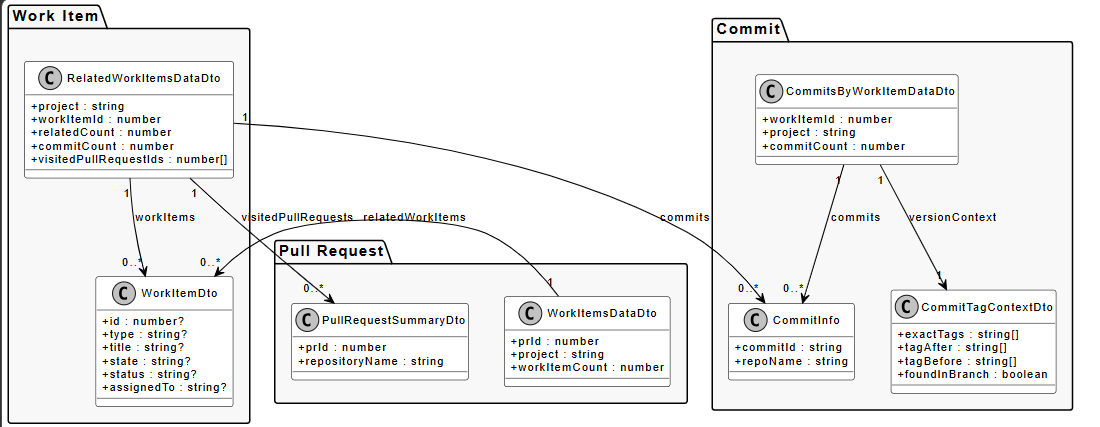
\includegraphics[width=1\linewidth]{img/archi/workitems_pr_commit_class_diag.png}
    \caption{Backend class diagram for the work item, pull request, and commit modules}
    \label{fig:backend-workitem-pr-commit-class-diagram}
\end{figure}

\begin{figure}[H]
    \centering
    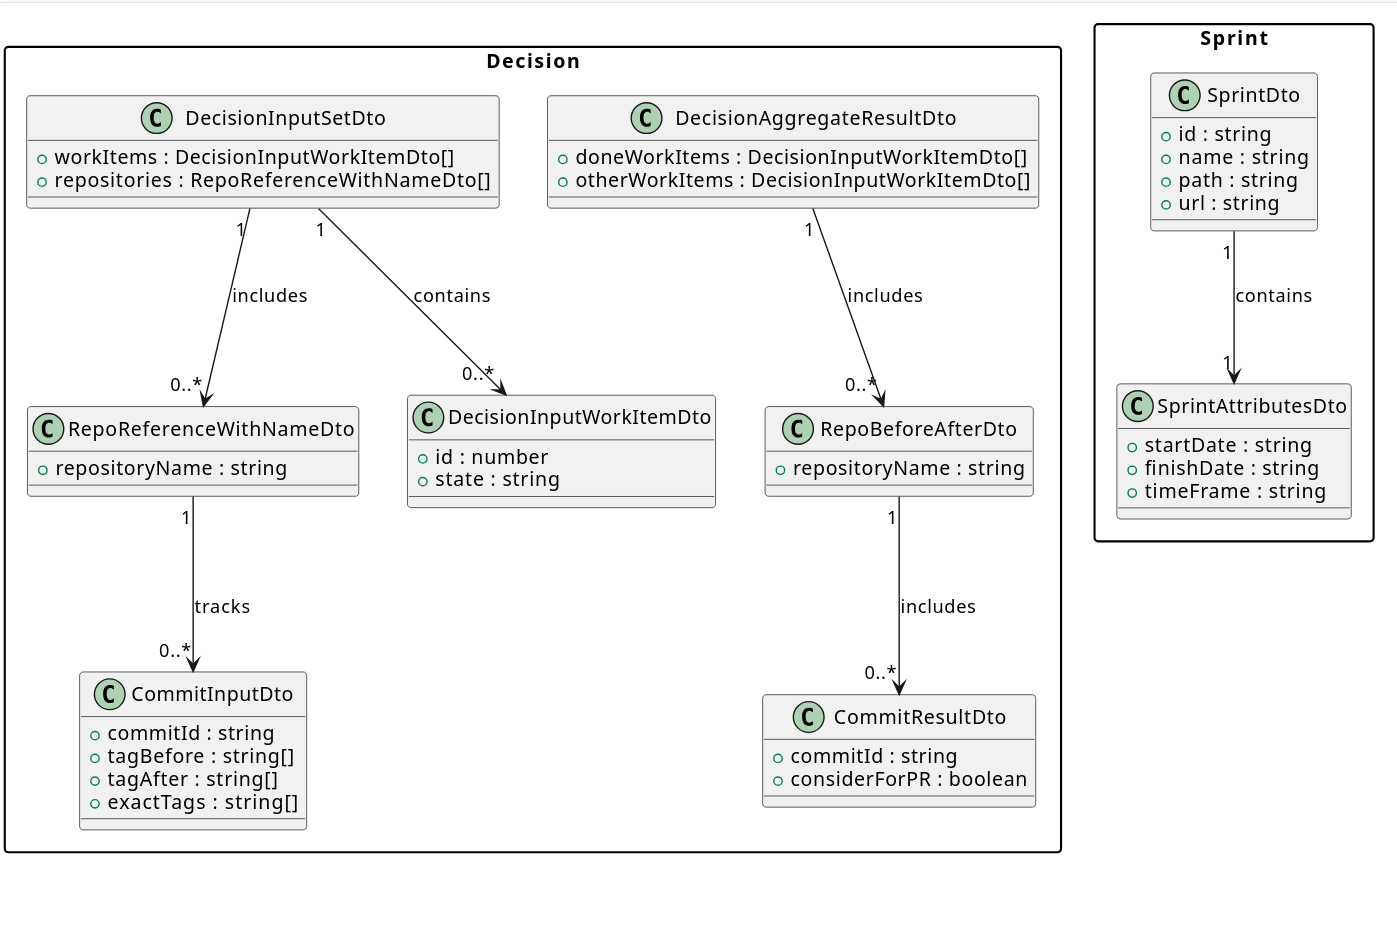
\includegraphics[width=1\linewidth]{img/archi/sprint_decision_class_diag.png}
    \caption{Backend class diagram for the sprint and decision modules}
    \label{fig:backend-sprint-decision-class-diagram}
\end{figure}

\subsection{API Contract Design}

The backend exposes a set of RESTful endpoints that support both single and
batch traceability analysis with a consistent response model.

\begin{description}
  \item[Single related endpoint]
  \texttt{/workitem/:id/related}

  Returns a traceability graph centered on a single root work item.

  \item[Batch related endpoint]
  \texttt{/workitem/related}

  Returns an aggregated, deduplicated graph for multiple root items.

  \item[Tasks stream endpoint]
  \texttt{/workitem/tasks/stream}

  Streams processing results progressively using Server-Sent Events (SSE).

  \item[PR-to-work-items endpoint]
  \texttt{/pullrequests/:prId/workitems}

  Retrieves work items linked to a given pull request.

  \item[Sprint listing endpoint]
  \texttt{/sprint?project=...}

  Returns the iterations available for a project.

  \item[Sprint work-items endpoint]
  \texttt{/sprint/:sprintId/work-items?project=...}

  Returns work items for a given sprint and supports lazy loading in the UI.

  \item[Commit tag batch endpoint]
  \texttt{/commits/tags/batch}

  Enriches commit references with repository tag metadata.

  \item[LLM commit review endpoint]
  \texttt{/commits/hf/review}

  Generates an AI-assisted review for a selected commit using repository and
  commit context.
\end{description}

The DTO strategy prioritizes:
\begin{itemize}
  \item stable response contracts between the backend and its consumers;
  \item best-effort metadata enrichment (e.g., repository names for visited PRs);
  \item a clear separation between operational traceability contracts and
  optional AI-generated review payloads;
  \item explicit counters and trace metadata for UI sorting and interpretation.
\end{itemize}

\subsection{Implementation Characteristics}

\begin{itemize}
  \item graph traversal with visited-state tracking to prevent cycles;
  \item request-scoped caching and batched retrieval to reduce external API load;
  \item normalization of external payloads before propagation between services;
  \item structured logging to support diagnostics and operational monitoring.
\end{itemize}

\subsection{Sequence and Processing Flows}

Backend processing is built around orchestration pipelines where each service
builds on the output of the previous stage.

\begin{itemize}
  \item \textbf{Single-root flow:} resolve the root work item, traverse related
  nodes, enrich pull requests and commits, return a normalized graph.
  \item \textbf{Batch flow:} run multi-root traversal with deduplication and
  consolidated counters.
  \item \textbf{Sprint exploration flow:} load project sprints, lazily fetch
  sprint work items, then forward selected items to the batch flow.
  \item \textbf{Commit tag flow:} resolve tag context in batch, grouped by
  repository, using a latest-tag strategy.
  \item \textbf{LLM review flow:} collect commit metadata and relevant file
  snapshots, augment the prompt with repository guidance, invoke the model,
  and return the generated review to the decision UI.
\end{itemize}

\begin{figure}[H]
  \noindent\makebox[\textwidth][c]{%
  
\includegraphics[width=\paperwidth,height=0.94\textheight,keepaspectratio]{"img/archi/single-root related-work-item processing.png"}
  }
  \caption{Sequence diagram for single-root related work-item processing}
  \label{fig:work-item-related-sequence}
\end{figure}

\begin{figure}[H]
\noindent\makebox[\textwidth][c]{%
  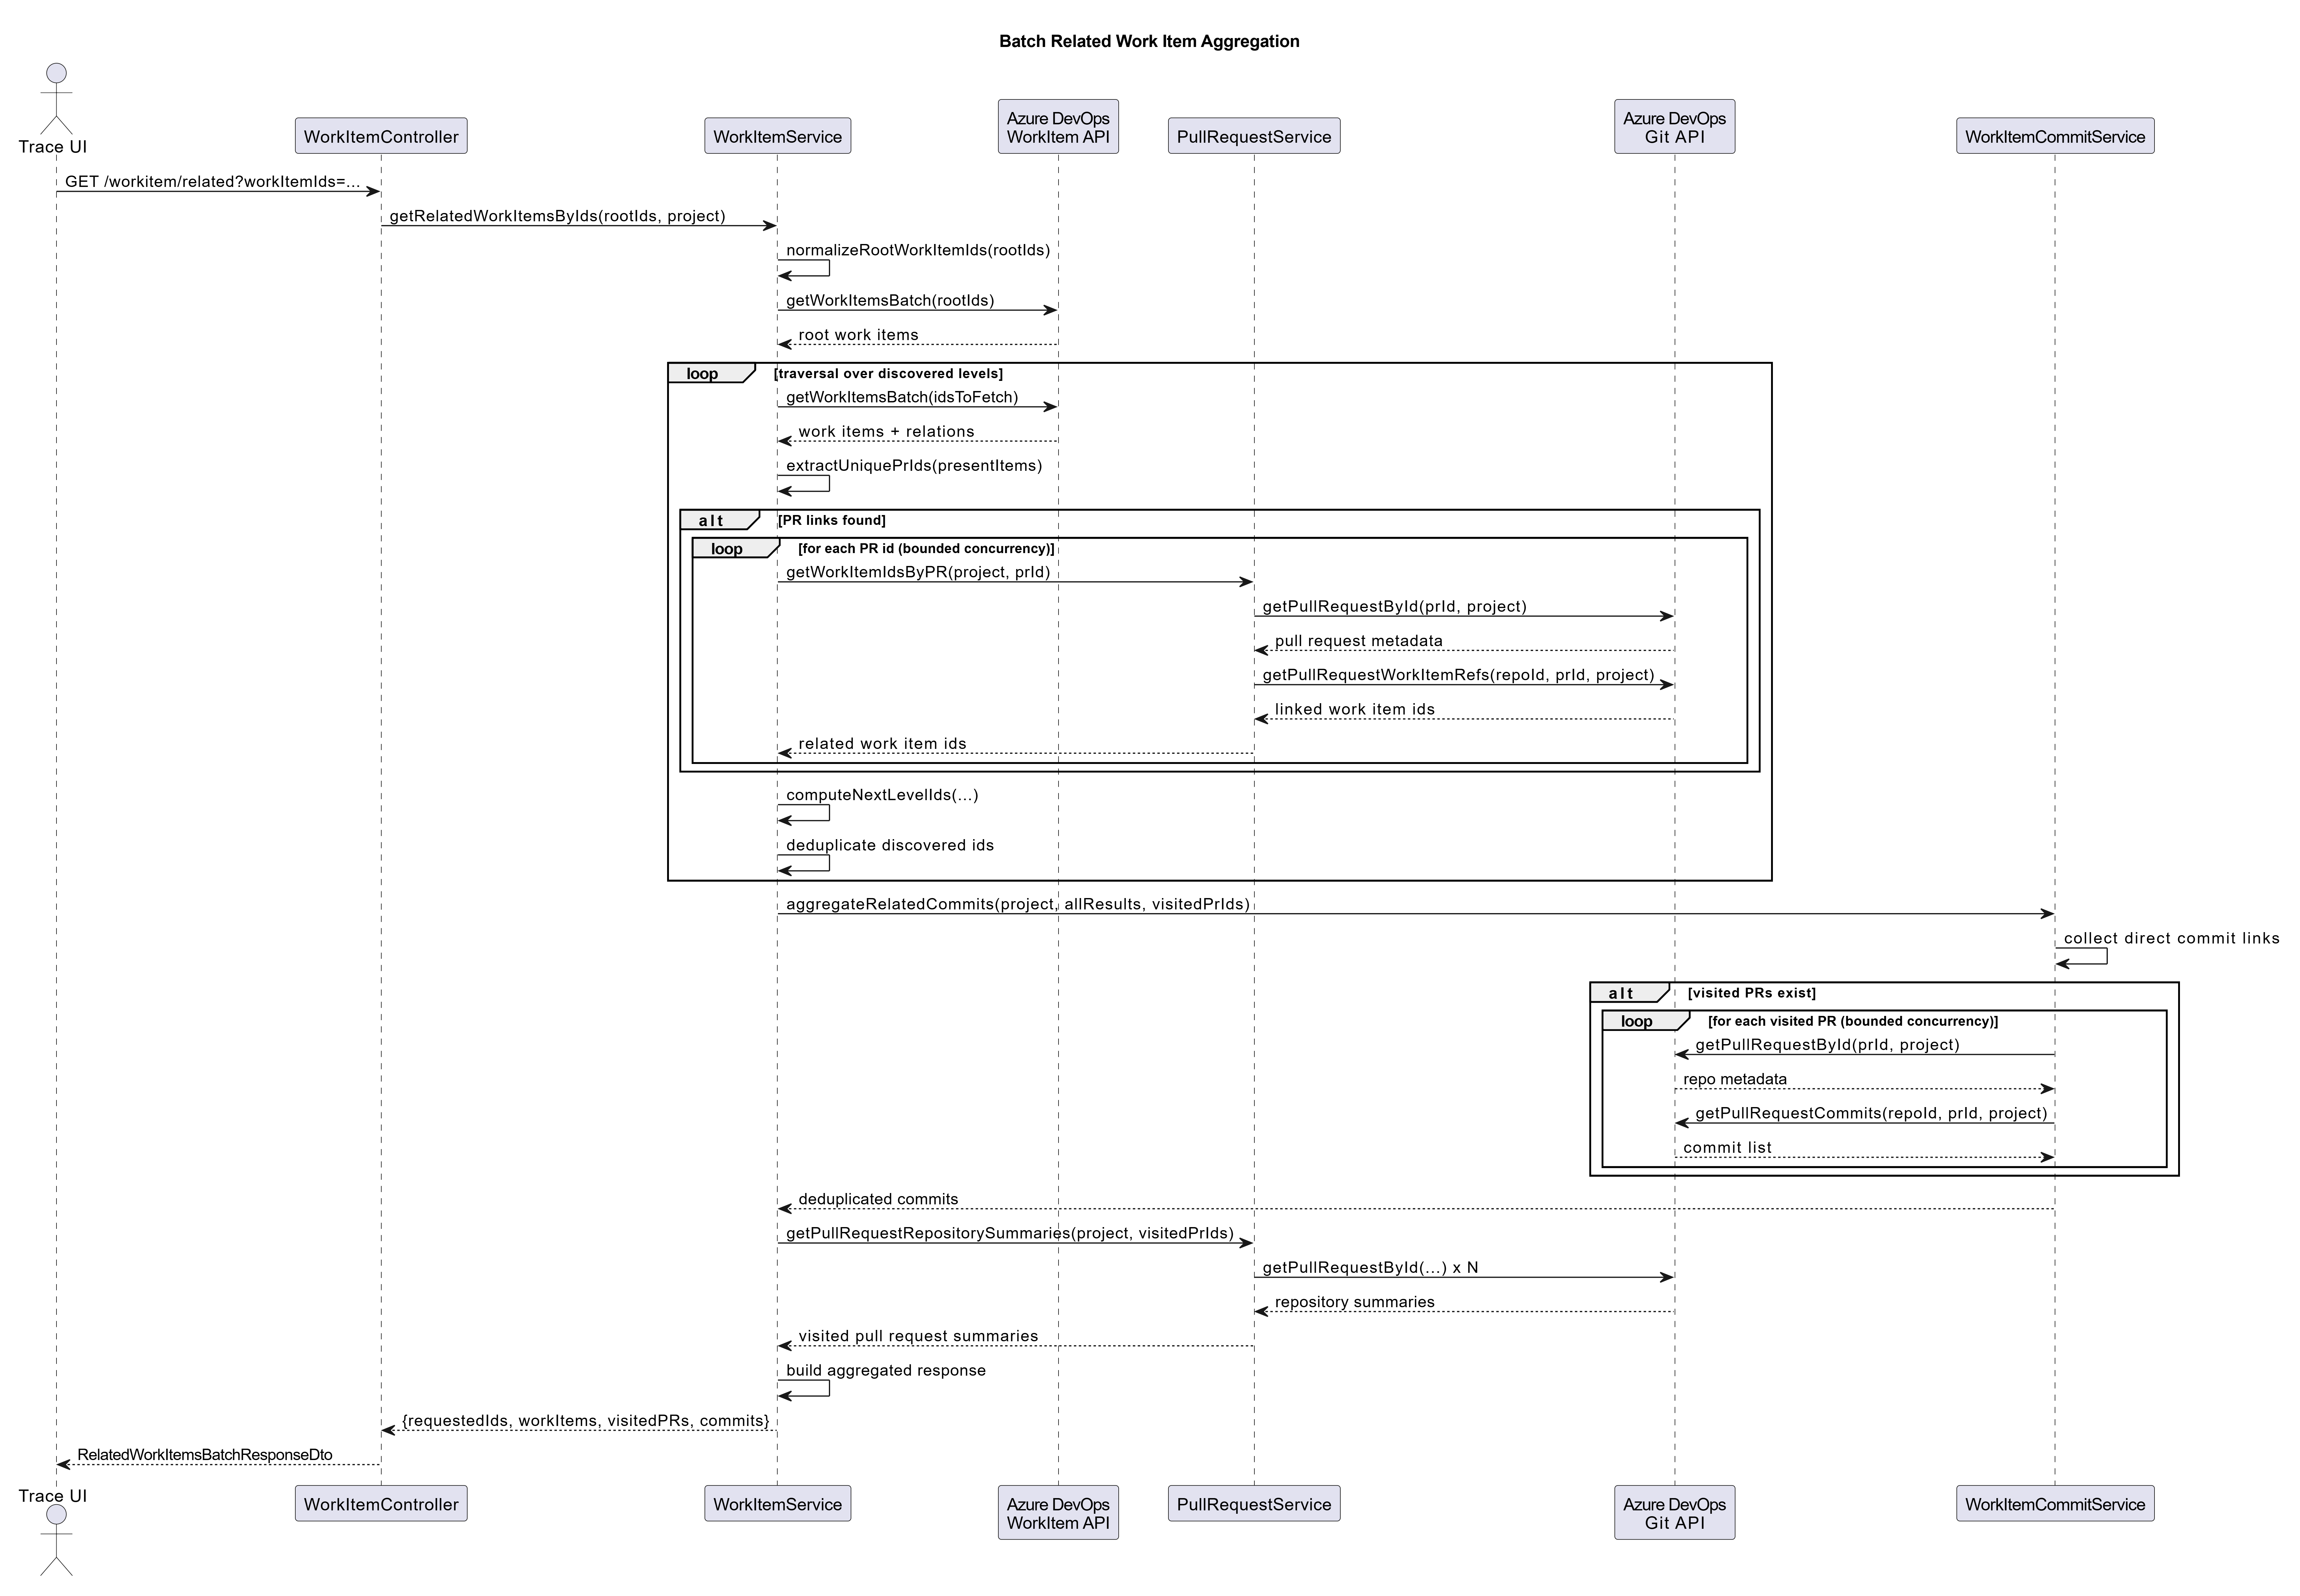
\includegraphics[width=\paperwidth,height=0.94\textheight,keepaspectratio]{img/archi/BatchRelatedWorkItem.png}
}
  \caption{Sequence diagram for batch related work-item aggregation}
  \label{fig:work-item-batch-sequence}
\end{figure}

% ──────────────────────────────────────────────────────────────────────────────
\section{UI Implementation}

\subsection{UI Architecture and Main Surfaces}

The UI layer is the main entry point to the traceability system. It is
organized around route-driven views that map to the key analysis scenarios,
with a shared state and API integration layer handling requests, progressive
loading, and result display.

\begin{itemize}
  \item \textbf{RelatedWorkItemTrace:} single-root analysis screen for
  exploring one work item and its related artifacts.
  \item \textbf{BatchWorkItemTrace:} selection and loading screen for
  progressively collecting candidate work items through SSE streaming.
  \item \textbf{SprintWorkItemsView:} planning-oriented screen for loading
  sprints, lazily fetching their work items, and preparing cross-sprint
  selections.
  \item \textbf{BatchRelatedWorkItemTrace:} aggregated result screen showing
  the consolidated output of multi-root analysis with commit and repository
  context.
  \item \textbf{DecisionDashboard:} decision and promotion screen extended
  with commit-level LLM review actions.
\end{itemize}

\begin{figure}[H]
\noindent\makebox[\textwidth][c]{%
  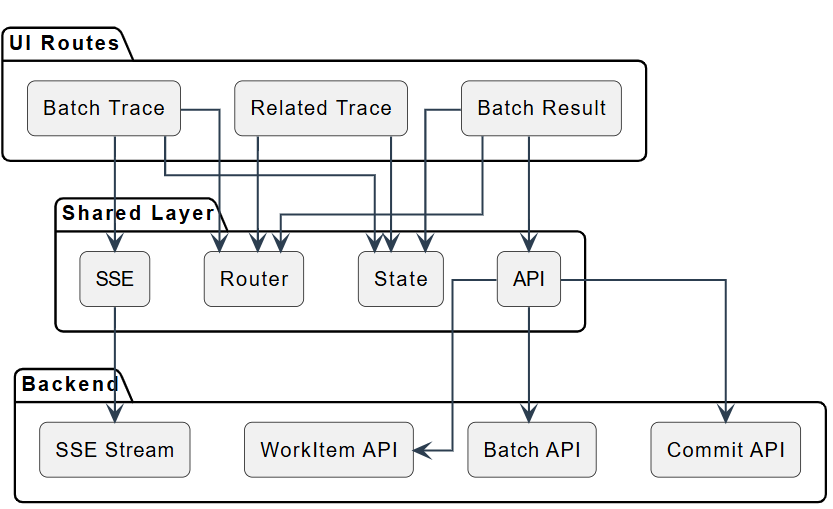
\includegraphics[width=\paperwidth]{img/figures/uiroutes.png}
}
  \caption{UI route and component architecture for traceability workflows}
  \label{fig:ui-route-component-diagram}
\end{figure}

\subsection{UI Data Flow and Backend Integration}

The UI communicates with the backend through a dedicated trace API layer and
maps backend contracts to typed frontend models.

\begin{itemize}
  \item Single analysis uses \texttt{/workitem/:id/related}.
  \item Batch task loading consumes \texttt{/workitem/tasks/stream} via SSE.
  \item Sprint exploration calls \texttt{/sprint} and
  \texttt{/sprint/:sprintId/work-items} with lazy retrieval per expanded sprint.
  \item Batch result enrichment uses \texttt{/commits/tags/batch} grouped by
  repository.
  \item Commit-level review actions call \texttt{/commits/review} from the
  decision dashboard when the operator requests an AI-generated assessment.
  \item Authentication failures trigger a controlled redirect when the backend
  returns an unauthorized response.
\end{itemize}

\begin{figure}[H]
  \noindent\makebox[\textwidth][c]{%
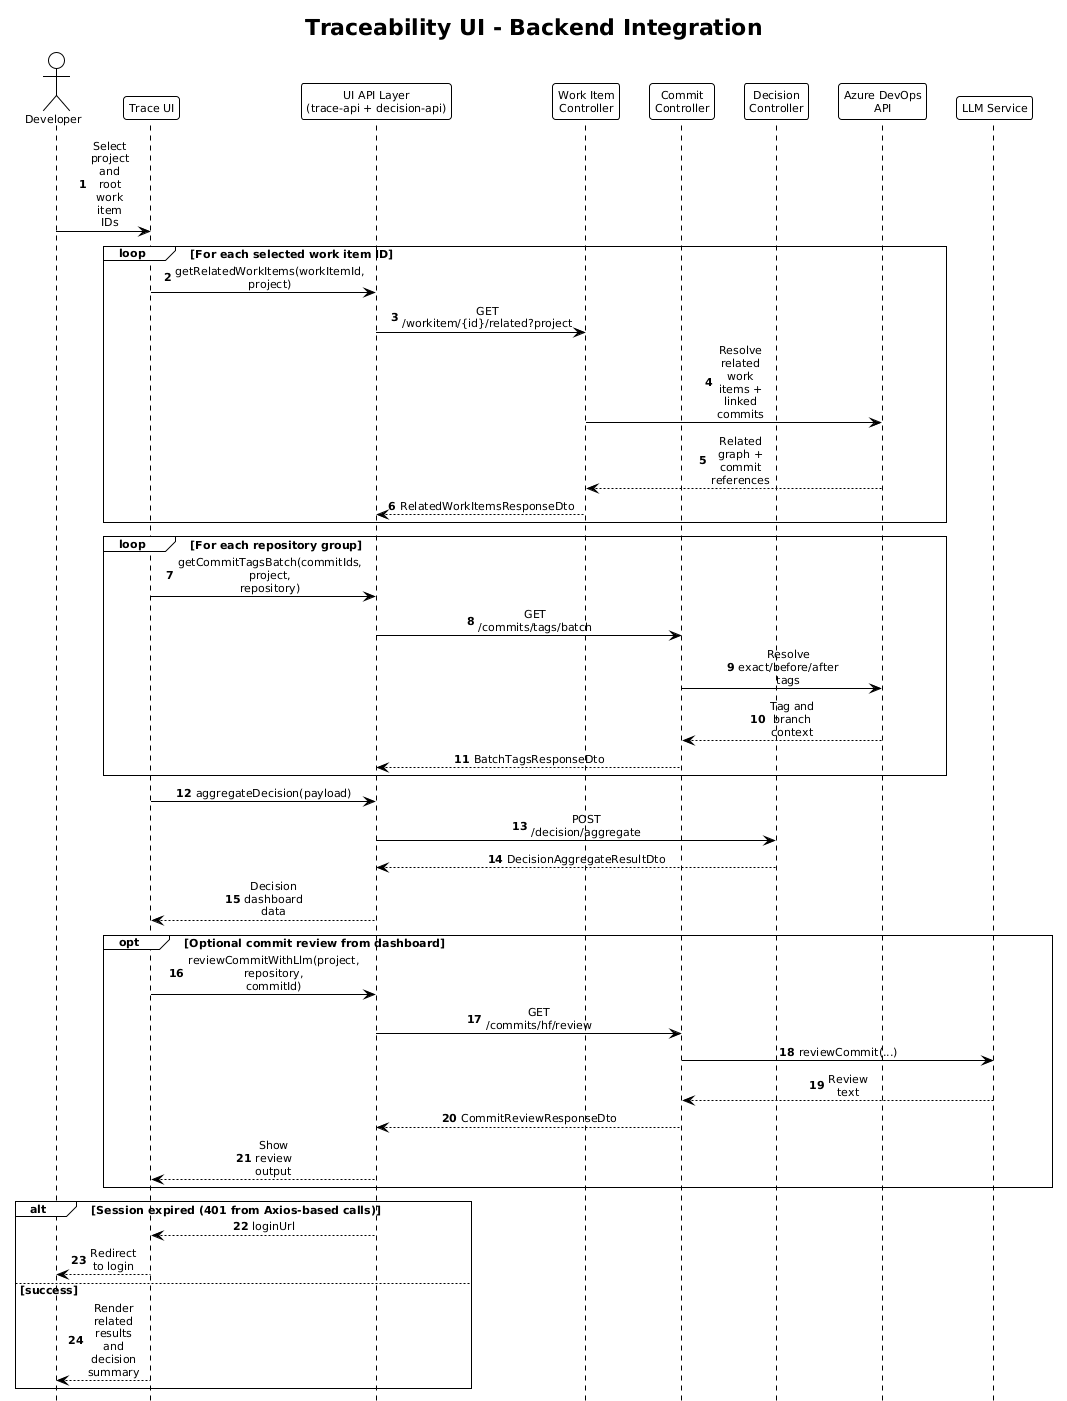
\includegraphics[width=\paperwidth,height=0.90\textheight,keepaspectratio]{img/archi/backend_uiflow.png}}
\caption{Sequence diagram for UI and backend integration in trace workflows}
\label{fig:ui-backend-integration-sequence}
\end{figure}


\subsection{UI Operational Considerations}

\begin{itemize}
  \item progressive loading to keep batch interactions responsive;
  \item consistent result ordering based on traceability counters;
  \item graceful rendering when enrichment metadata is partially unavailable.
\end{itemize}

\subsection{Screens and UI Walkthrough}

\subsubsection{Batching Work Items}

This screen is used to select multiple work items for batch processing and kick
off a batched traceability run. Selection is flexible --- single items, multiple,
or all at once --- and run progress is shown progressively using Server-Sent
Events (SSE). The screen includes quick filters and tools for prioritizing
candidates before downstream aggregation.

\begin{figure}[htbp]
\noindent\makebox[\textwidth][c]{%
  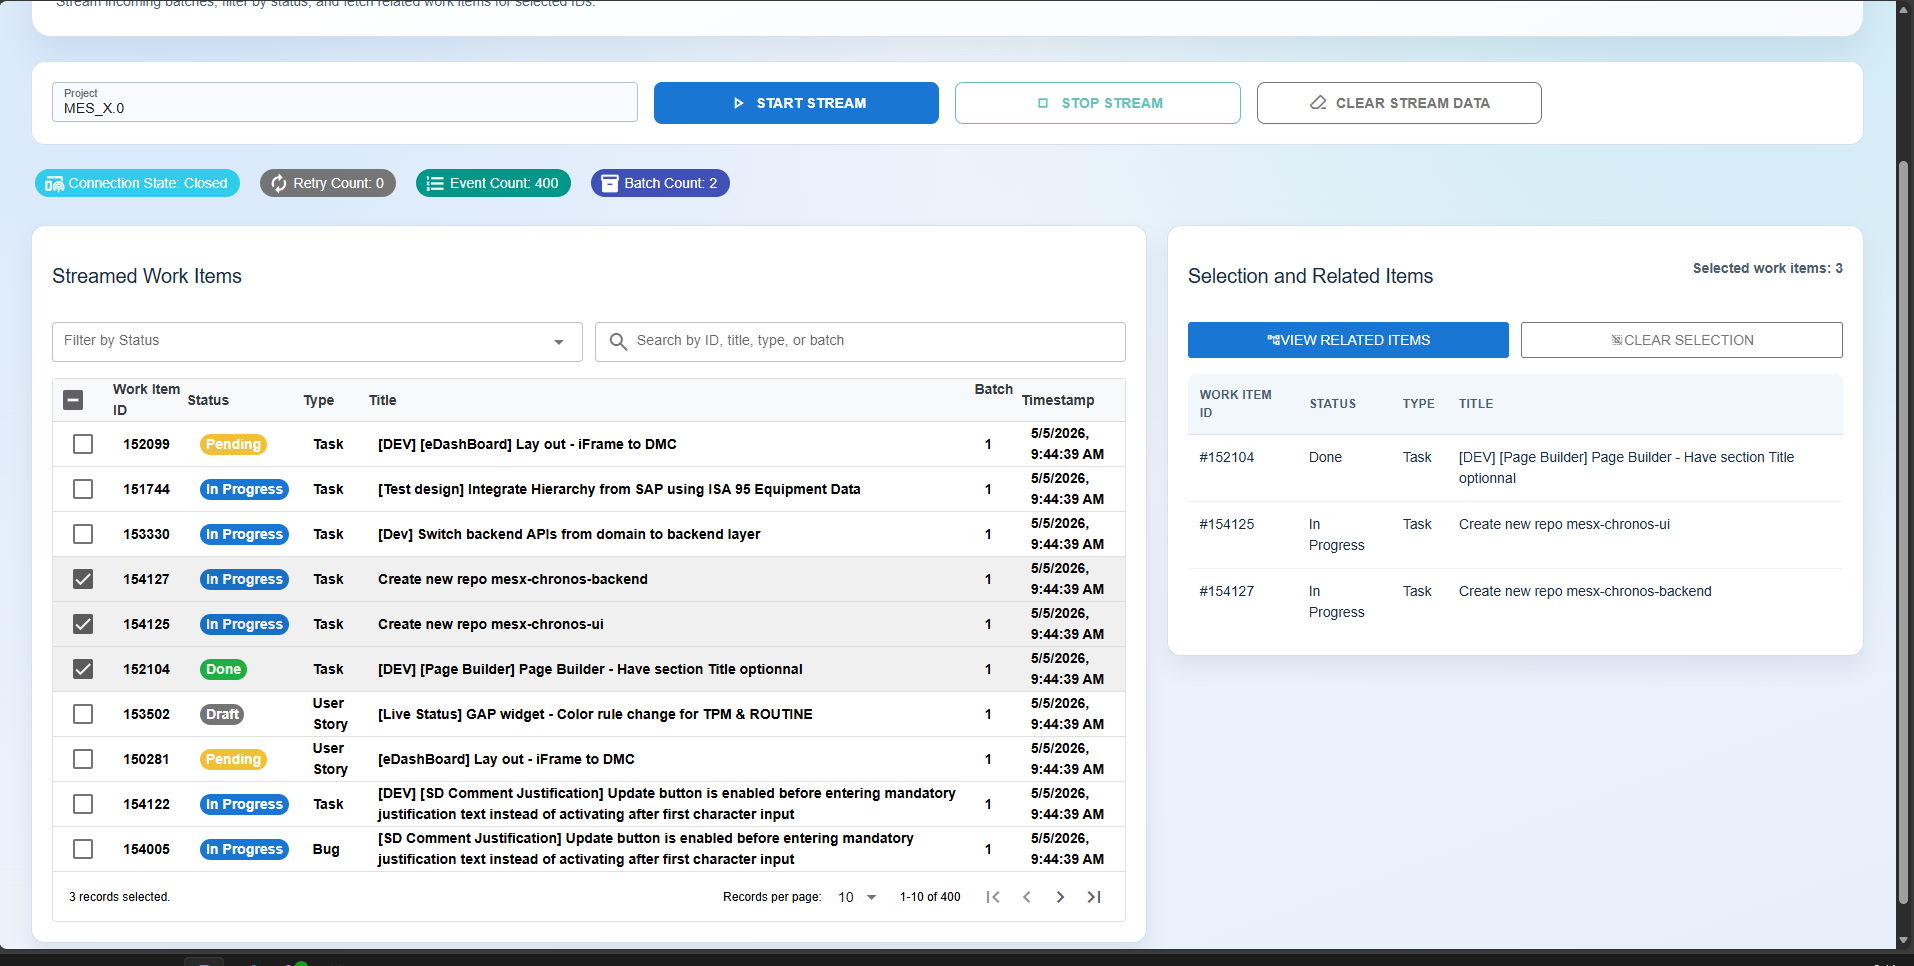
\includegraphics[width=\paperwidth]{img/figures/ui-batch-task-screen.png}
}
  \caption{Batching Work Items -- selection and SSE-driven progress}
  \label{fig:batching-wi}
\end{figure}

\subsubsection{Get Related}

The "Get Related" flow has two complementary screens:

\begin{figure}[htbp]
\noindent\makebox[\textwidth][c]{%
  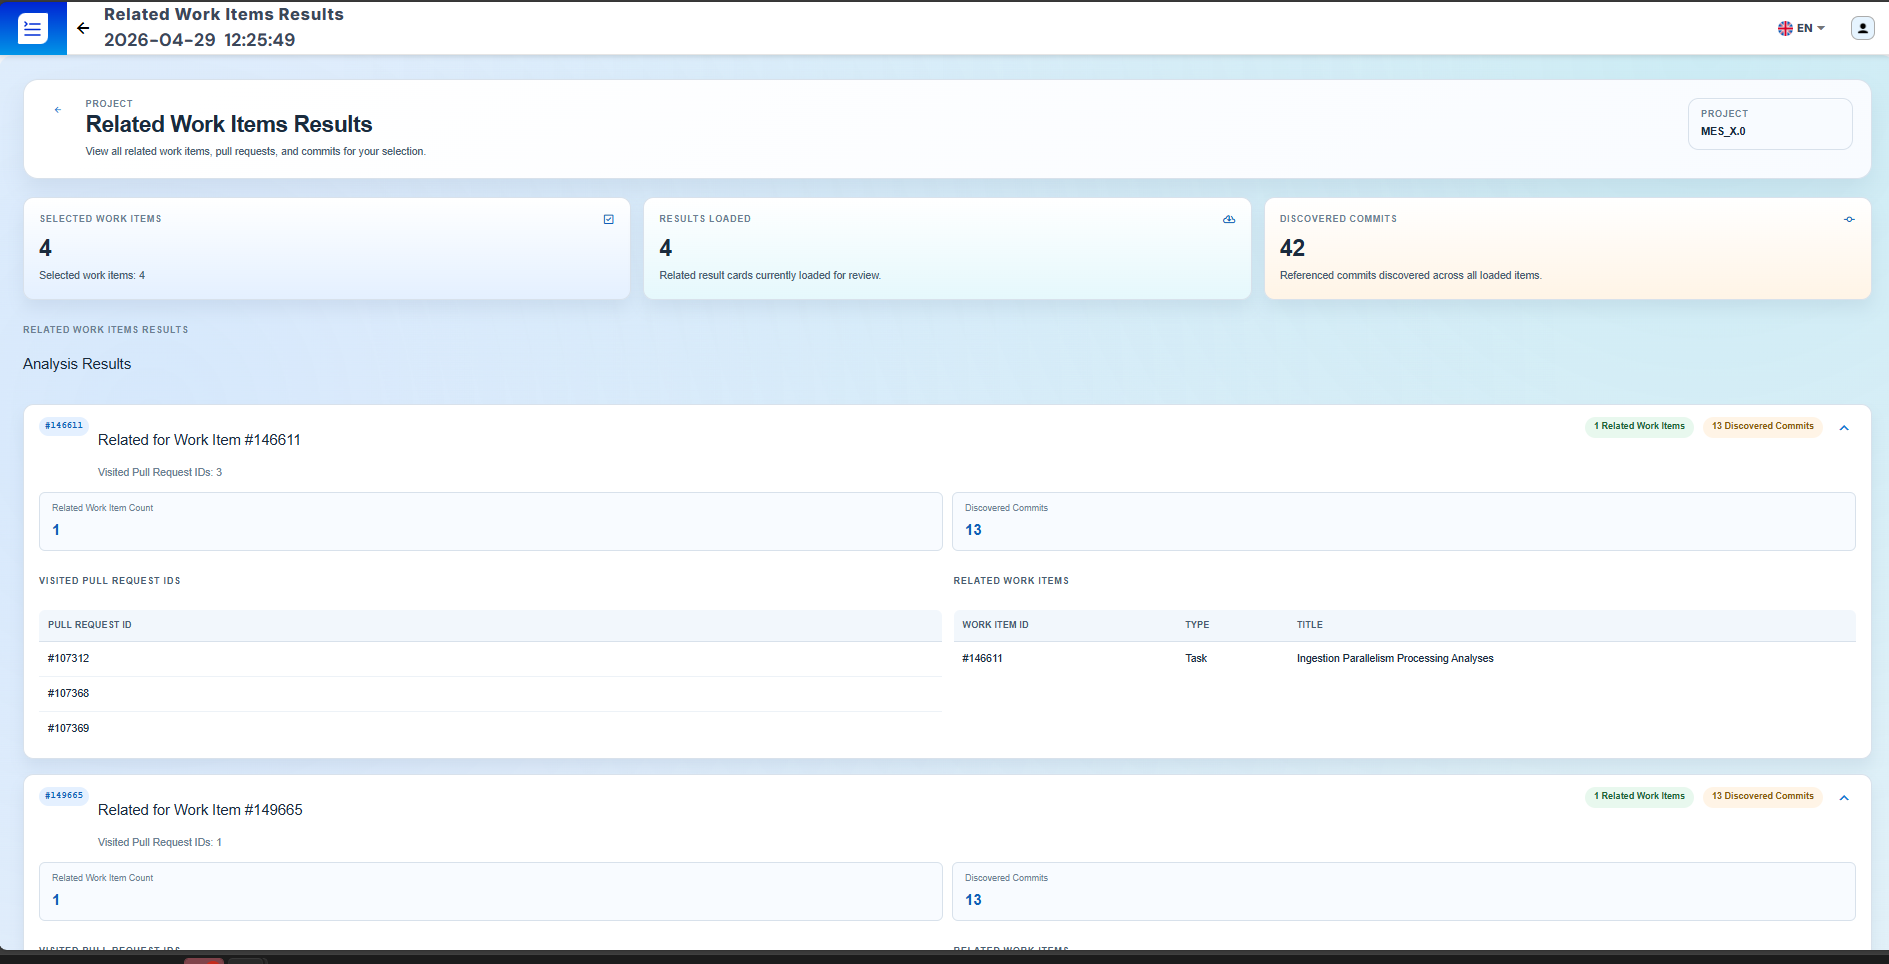
\includegraphics[width=\paperwidth]{img/figures/related-workitem1.png}
}
  \caption{Related Work Item -- single-root traceability graph view}
  \label{fig:related-workitem}
\end{figure}

The Related Work Item view shows a single root work item and its connected
graph (pull requests, commits, branches, tags). Nodes can be expanded and
inspected, and the operator can drill down to commit or PR level.

\begin{figure}[htbp]
\noindent\makebox[\textwidth][c]{%
  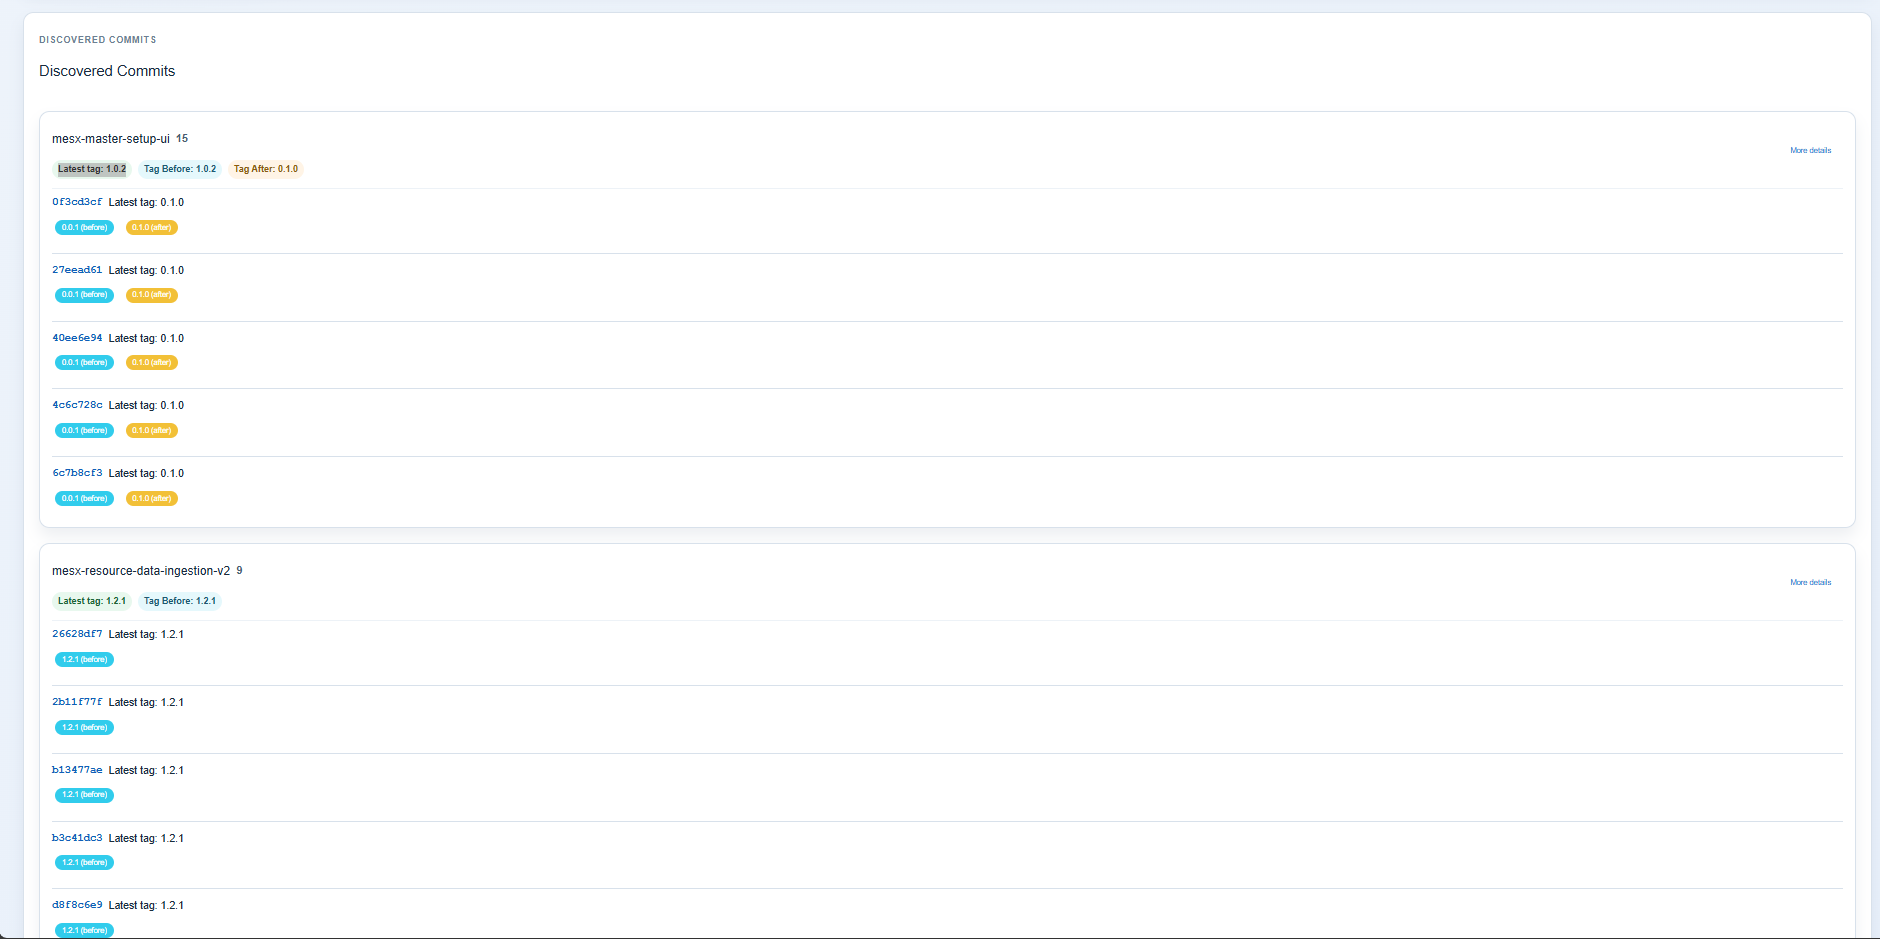
\includegraphics[width=\paperwidth]{img/figures/discovered-commits.png}
}
  \caption{Discovered Commits -- commits found during traversal}
  \label{fig:discovered-commits}
\end{figure}

The Discovered Commits screen lists commits found during traversal along with
contextual metadata: branch, tags, and associated work items. This view is
useful for verifying commit-to-work-item linkage and checking tag context
before any automated decisions are made.

\subsubsection{Sprint Work Items}

The Sprint Work Items screen provides a planning-driven entry point to the
traceability workflow. Rather than starting from manually entered identifiers,
the operator loads the sprint list for a project and expands individual sprint
cards to lazily fetch their work items. Selected items are kept across loaded
sprints and can be forwarded directly to the batch analysis flow.

\subsubsection{Decision}

The Decision section provides summarized outputs to guide promotion actions.
It contains two key screens:

\begin{figure}[htbp]
\noindent\makebox[\textwidth][c]{%
  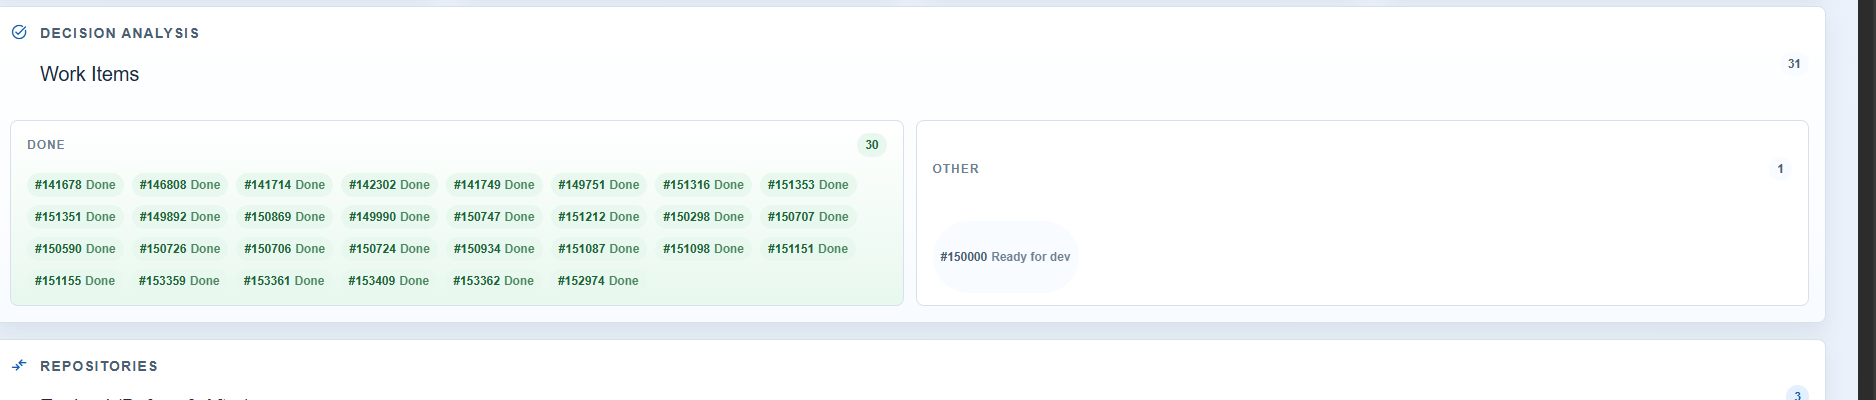
\includegraphics[width=\paperwidth]{img/figures/decision-wi-state.png}
}
  \caption{Decision -- work items grouped by state (Done vs. Other)}
  \label{fig:decision-wi-state}
\end{figure}

The first Decision view groups work items by state (for example, \texttt{Done}
vs \texttt{Other}) so operators can quickly see which items are ready for
promotion and which still need attention.

\begin{figure}[htbp]
\noindent\makebox[\textwidth][c]{%
  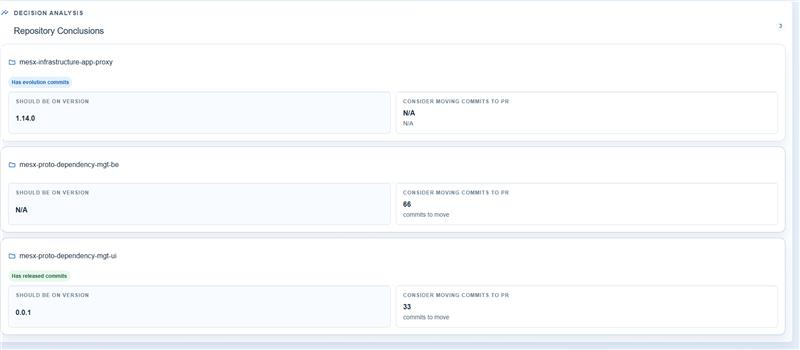
\includegraphics[width=\paperwidth]{img/figures/decision-repo-tags.jpg}
}
  \caption{Decision -- repository view with expected tags for promotion}
  \label{fig:decision-repo-tags}
\end{figure}

The repository/tags screen shows, per repository, the commits and expected tags
(before/after/exact) that the system identified. From here, an operator can
select a candidate work item and trigger a promotion workflow (for example:
move a work item to production) after reviewing tag context. The same screen
also exposes an LLM review action on eligible commits, allowing the operator
to request an AI-generated assessment before making a final decision.

% ──────────────────────────────────────────────────────────────────────────────
\section{Docker Orchestration and Deployment}

\subsection{Service Orchestration Model}

The backend runtime is packaged as an isolated service with clearly defined
integration boundaries.

\begin{itemize}
  \item The backend container exposes REST/SSE APIs on the configured runtime port.
  \item Runtime configuration and secrets are injected through environment
  variables and externalized config files.
  \item The backend accesses Azure DevOps Work Item and Git APIs over HTTPS.
\end{itemize}

\subsection{Operational Dependencies}

\begin{itemize}
  \item CI/CD pipeline for image build and deployment validation.
  \item Optional caching layer through internal cache services.
  \item Secrets and environment values injected at runtime.
\end{itemize}

\subsection{Deployment Objectives}

\begin{itemize}
  \item reproducible execution locally and in CI;
  \item independent versioning and rollout of backend artifacts;
  \item reduced deployment risk through clear component ownership.
\end{itemize}

% ──────────────────────────────────────────────────────────────────────────────
\section{Quality, Security, and Operational Considerations}

\subsection{Testing and Validation}

Validation was carried out at multiple levels to ensure the delivered solution
matched the requirements defined earlier in this report.

\begin{itemize}
  \item Backend unit tests covered controller and service behavior, especially
  work item traversal, commit resolution, and DTO mapping.
  \item End-to-end tests validated the main API flows and confirmed the
  frontend correctly consumed the backend contracts.
  \item Frontend quality checks combined linting, style validation, and manual
  testing of the main traceability views and the decision dashboard.
  \item Cross-layer checks ensured that streaming behavior, repository grouping,
  and decision outputs remained consistent from backend to UI.
\end{itemize}

\subsection{Developed Tests}

The test effort focused on validating the most critical traceability services
and API contracts used by the UI.

\begin{itemize}
  \item \textbf{Backend unit tests (Jest):} implemented for the Work Item,
  Commit, and Sprint modules, including controller and service-level behavior.
  \item \textbf{Backend utility tests:} added for tag-selection logic used by
  repository context enrichment.
  \item \textbf{Backend API end-to-end test:} implemented under the
  \texttt{test/} suite to validate core HTTP integration behavior.
  \item \textbf{Frontend validation:} performed through linting, static checks,
  and manual scenario-based verification of key traceability screens.
\end{itemize}

\textbf{Quality controls:}
\begin{itemize}
  \item controller-level input validation and typed DTO contracts;
  \item service-level tests for traversal, tag selection, and data normalization;
  \item regression-focused tests for traversal and normalization behavior.
\end{itemize}

\textbf{Security and runtime controls:}
\begin{itemize}
  \item secure communication for all backend integrations;
  \item managed access to Azure DevOps external APIs;
  \item structured logging to support incident analysis and diagnostics.
\end{itemize}

% ──────────────────────────────────────────────────────────────────────────────
\section{AI-assisted Development and Review}

AI-assisted tools were used throughout the project to support both backend and
frontend work. The goal was not to replace engineering decisions, but to speed
up repetitive tasks, improve review coverage, and encode project-specific
conventions.

The application also ships an operational LLM capability within the backend
itself. The Commit module delegates review requests to a dedicated LLM module
that builds prompts from Azure DevOps commit metadata, selects a small set of
relevant changed files, injects repository instructions and skill guidance, and
calls an external model to produce a structured review. This review is then
surfaced in the decision dashboard, so release analysis can be complemented by
code-level observations when needed.

Both repositories keep their automation artifacts inside the codebase. On the
backend, the \texttt{.github/agents/} directory defines dedicated roles such as
architect, implementer, reviewer, and QA agent. On the frontend,
\texttt{.github/agents/}, \texttt{.github/instructions/}, and
\texttt{.github/skills/} capture UI guidelines, review rules, and reusable
workflows for Vue, Quasar, styling, and quality checks. Keeping these files
versioned alongside the source code makes the automation explicit, reviewable,
and reproducible.

In practice, these agents assisted with code drafting, refactoring, test
scaffolding, documentation, and architecture reviews. The instruction files
helped enforce conventions such as typed contracts, logging discipline,
component structure, localization, and style consistency. On the frontend they
reinforced guardrails around Vue Composition API usage, token-based styling,
and UI quality. On the backend they kept DTO usage, controller-service
separation, and observability patterns consistent across the codebase.

All AI-generated suggestions went through human review. Proposed changes were
treated as drafts and validated through linting, SonarQube policies, tests, and
direct developer inspection before being merged. This made AI tools genuinely
useful across both development and runtime review support, while keeping
accountability, technical rigor, and architectural coherence firmly in human
hands.

% ──────────────────────────────────────────────────────────────────────────────
\section*{Conclusion}

The implementation produced a modular traceability platform combining a
graph-oriented backend, an operational frontend, and a deployment-ready runtime
configuration. The result replaces a manual, fragmented analysis process with a
structured workflow that is faster, easier to interpret, and better suited to
release preparation.

By combining layered design, iterative development, thorough validation, and
careful integration with Azure DevOps, the project built a maintainable
foundation for dependency analysis, release decision support, and future
expansion of the traceability scope.

\addcontentsline{toc}{section}{Conclusion}
\newpage

%% ════════════════════════════════════════════════════════════════════════════
%%  PART III — BACK MATTER
%% ════════════════════════════════════════════════════════════════════════════

%% ── General Conclusion ───────────────────────────────────────────────────────
\chapter*{General Conclusion}
\addcontentsline{toc}{chapter}{General Conclusion}
\markboth{General Conclusion}{General Conclusion}

This internship addressed a real problem: release preparation at Forvia
Informatique Tunisie was slow and spread across multiple Azure DevOps screens
with no unified view of how artifacts related to one another. The work covered
the full development cycle, from architecture and implementation to integration,
validation, and deployment.

The result is a modular traceability platform. The backend handles recursive
graph traversal across work items, pull requests, commits, and tags, with cycle
prevention, batch processing, and SSE streaming for progressive feedback. The
frontend gives operators a single flow from work item selection to
promotion-ready summaries, replacing a process that previously required
navigating several disconnected pages. A lightweight LLM review feature was
also integrated at commit level, keeping human validation as the final step.

Beyond the delivered features, the project confirmed a few practical lessons.
Incremental module delivery kept integration risks low. Strict DTO contracts
between backend and frontend prevented most regressions. Logging and structured
error handling proved essential once flows became multi-step and harder to
trace manually.

The platform is functional and deployed, but also designed to evolve. The
traceability graph it builds is machine-readable, which makes it a natural
foundation for a future planning assistant able to recommend repository change
paths and target versions directly from a work item or user story. That next
step would take MES-X from dependency exploration to guided release preparation,
which is the logical continuation of what was built here.
\newpage

%% ── Bibliography ─────────────────────────────────────────────────────────────
%% Uncomment and configure once your .bib file is ready:
%% \bibliographystyle{plain}          % or ieeetr, apalike, unsrt …
%% \bibliography{references}
%% \addcontentsline{toc}{chapter}{Bibliography}
%% \newpage

%% ── Appendices ───────────────────────────────────────────────────────────────
%% Uncomment if you have appendices:
%% \appendix
%% \include{chapters/appendix_a}

\end{document}